%*********************************************************************
% gdutthesis: 广东工业大学论文模板
% 2021/11/09 v0.1c
%
% 重要提示:
%   1. 请确保使用 UTF-8 编码保存
%   2. 请使用 XeLaTeX 或 LuaLaTeX 编译
%   3. 请仔细阅读用户文档和 Wiki
%   4. 修改、使用、发布本文档请务必遵循 LaTeX Project Public License
%   5. 不需要的注释可以尽情删除
%*********************************************************************
\documentclass[
  % type=doctor
  type=master
  % type=promaster
]{gdutthesis}

% 宏包在这里加载
\usepackage{siunitx}[=v2]
\usepackage{zhlipsum,lipsum}
\usepackage{algorithm}
\usepackage{algorithmic}

\gdutsetup{
  style = {
    cover           = {true},
    % cover           = {false},
    % font            = {garamond},
    % font            = {libertinus},
    % font            = {lm},
    % font            = {palatino},
    font            = {times},
    % font            = {times*},
    cjk-font        = {fandol},
    % cjk-font        = {founder},
    % cjk-font        = {mac},
    % cjk-font        = {sourcehan},
    % cjk-font        = {noto},
    % cjk-font        = {windows},
    % cjk-font        = {none},
    bib-backend     = {bibtex},
    % bib-backend     = {biblatex},
    bib-resource    = {gdutthesis-template.bib},
    bib-style       = {numerical},
    % bib-style       = {author-year},
    fullwidth-stop  = {mapping},
    % fullwidth-stop  = {catcode},
    % fullwidth-stop  = {false},
    hyperlink       = {color},
    % hyperlink       = {border},
    % hyperlink       = {none},
    hyperlink-color = {default},
    % hyperlink-color = {autumn},
    % hyperlink-color = {business},
    % hyperlink-color = {classic},
    % hyperlink-color = {elegant},
    % hyperlink-color = {fantasy},
    % hyperlink-color = {material},
    % hyperlink-color = {science},
    % hyperlink-color = {summer},
    % hyperlink-color = {graylevel},
    % hyperlink-color = {prl},
  },
  info = {
    title           = {多旋翼飞行器导航与控制算法研究},
    title*          = {Research on navigation and control algorithm of multi-rotor aircraft},
    date            = {2022/5/25},
    author          = {邓正雄},
    author*         = {Deng Zhengxiong},
    supervisor      = {鲁仁全\qquad 教授},
    supervisor*     = {Prof. Lu Renquan},
    supervisor-two  = {none},
    supervisor-two* = {none},
    department      = {自动化学院},
    department*     = {Automation},
    major           = {控制科学与工程},
    student-id      = {2111904069},
    chairman        = {赵六\qquad 教授},
    degree          = {工程硕士},
    degree*         = {Master of Engineering},
    keywords        = {多旋翼, 状态估计, 控制, 校准},
    keywords*       = {multi rotor, state estimation, control, calibration},
    secret-level    = {none},
  }
}


\begin{document}

\begin{abstract}
  由于多旋翼飞行器具有体积小、机动性强、悬停能力强等优点,其在监视、搜索和救援等场景有很好的应用前景。
  在这些场景中,飞行器必须能够自主飞行,以尽量减少操作员的工作量。
  随着近年来机器人技术的快速发展,能够实现自主飞行的飞行器已经广泛应用于各种场景当中。
  但是,在传感器受干扰、使用低成本传感器情况下进行自主飞行会带来一些具有挑战性的工程问题。
  解决这些工程问题需要对估计、校准、控制等算法进行综合设计。
  其中,状态估计是自主飞行的首要和最关键的组成部分。
  本文提出了以状态估计为重点的方法和系统设计,使多旋翼飞行器能够在传感器信息受限及干扰情况下自主飞行。
  首先,我们提出了预测-修正-延时融合框架,以处理多频率多延时的传感器系统。
  然后,我们对每个传感器的特性进行研究,针对磁场干扰及运动加速度补偿进行优化处理,以提高系统的鲁棒性。
  其次,我们进一步优化了IMU校准算法,提出了新的最优阈值的算法,改进了参数估计算法,提高了IMU本身输出数据的精度。
  最后,我们整合了控制算法,形成一个完整的飞行控制系统。
  本文提供了大量的实验结果。
  最后,我们提出了未来的研究方向。
\end{abstract}

\begin{abstract*}
  Micro aerial vehicles (MAVs) are ideal platforms for surveillance and search and rescue due to their small size, superior mobility, and hover capability.
  In such missions, it is essential that the MAV is capable of autonomous flight to minimize operator workload.
  With the rapid development of robot technology in recent years, aircraft capable of autonomous flight has been widely used in various scenarios.
  Autonomous navigation in sensor interference, the use of low-cost sensors gives rise to challenging engineering
  problems.
  We require an integrated approach to estimation, calibration, and control to solve these engineering problems.
  Among these, state estimation is the first and most critical component for autonomous flight.   
  In this thesis, we present methodologies and system designs, with a focus on state estimation, that enable a light-weight off-the-shelf quadrotor MAV to autonomously navigate in the case of sensor information limitation and interference.
  We start by presenting a prediction-correction-delay fusion framework to deal with multi-frequency and multi-delay sensor systems.
  We then investigate the characteristics of each sensor and optimize the magnetic field interference and motion acceleration compensation to improve robustness.
  we further optimize the IMU calibration algorithm and propose a new optimal threshold algorithm to improve the accuracy of IMU output data.
  Finally, we integrated the control algorithm into a complete flight control system.  	
  Extensive experimental results are presented throughout the thesis. 
  We conclude by proposing future research opportunities.
\end{abstract*}

\begin{notation}
  $E$ & 能量 \\
  $F$ & 推力
\end{notation}

\gduttableofcontents

\mainmatter

\gdutchapter{绪论}{Introduction}

\gdutsection{研究背景及意义}{Background and significance of research}
由于多旋翼飞行器具有体积小、机动性强、悬停能力强等优点,其在监视、搜索和救援等场景有很好的应用前景。
在这些场景中,飞行器必须能够自主飞行,以尽量减少操作员的工作量。
随着近年来机器人技术的快速发展,能够实现自主飞行的飞行器已经广泛应用于各种场景当中,如航空摄影、交通运输和智能农业。
除了上述应用场景外,在人员和地面机器人难以接近或危险复杂环境中,飞行器在监视、搜索和救援任务中具有巨大的潜力。
在这样的环境中,飞行器作业的主要挑战是传感器干扰和传感器本身数据精度低。
传感器干扰包括但不限于气压计干扰、磁场干扰、GPS信号异常。
由于使用低成本的传感器,传感器本身的数据精度限制了导航系统的精度。
到目前为止,研发一个多旋翼飞行器,并能够在这样的环境中快速自主飞行,仍然会带来挑战性的工程问题,需要对估计、校准、控制等算法进行综合设计。
因此,本文将对状态估计、校准和控制这三个问题进行研究。
其中,状态估计是自主飞行的首要和最关键的组成部分。

\gdutsection{国内外研究现状}{Analysis of the research status at home and abroad}
近年来,人们对应用在多旋翼飞行器的导航与控制系统进行了广泛的研究。
我们首先回顾了多旋翼飞行器发展过程中出现的一些研究问题。
我们在本节回顾关于每个问题及其相关领域的文献。
接下来我们对估计、校准、控制三个问题进行回顾。

\gdutsubsection{传感器融合}{Sensor fusion}
估计一个刚体的状态(即位置和姿态)是机器人鲁棒和高性能控制的关键要求。
机器人的状态估计是一个非线性的问题,使用的传感器通常包含了非高斯噪声\cite{baldwin2009inertial}。
一种标准的方法是使用扩展的随机线性估计技术\cite{lefferts1982kalman,barshan1995inertial}。
另一种方法是使用确定性互补滤波器和非线性观测器设计技术\cite{zimmermann1992high,baerveldt1997low,vik2001nonlinear}。
在随机线性估计技术中,应用于姿态估计问题的主要算法是扩展卡尔曼滤波(EKF)型方法。
粒子滤波器也被认为是处理非线性的一种方法\cite{cheng2004particle}。
由于状态空间的非线性而遇到困难,EKF表现出非鲁棒性和不稳定性\cite{crassidis2007survey}。
相反,非线性观测器利用基础几何来解释问题本质中的非线性。
因此,非线性观测器相比于EKF鲁棒性更强,并具有可证明的几乎全局稳定的性质\cite{thienel2003coupled,mahony2008nonlinear,lageman2009gradient,hua2010attitude,vasconcelos2010nonlinear}。
对于姿态问题,Mahony等人利用所有旋转的特殊正交群SO(3)的基本李群结构推导了一个互补非线性姿态观测器,并证明了误差系统的几乎全局稳定性\cite{mahony2008nonlinear}。
磁场干扰会影响横滚角和俯仰角的估计。
Hua等人考虑了输入信号的解耦,以确保滚转和俯仰估计不受磁场干扰的影响,这代表了显式互补滤波器标准实现的一个重要修改,以提高姿态估计的整体质量\cite{hua2011nonlinear}。
大多数现有的姿态观测器/滤波器都依赖于小加速度假设(即$\dot{v}<<g$),因此重力方向测量可以近似于加速度计测量。
然而,对于许多垂直起降飞行器在快速运动中,飞行器的线性加速度通常是较大的,可能会在姿态估计上产生很大的误差。
对于较大的线性加速度,可以将GPS线速度的测量值与加速度计的测量值相结合来估计飞行器的加速度,从而提高姿态估计的精度。
Hua等人提出了GPS辅助姿态观测器\cite{hua2010attitude}。
以上提到的所有的观测器设计方法都要求对系统的当前输出和输入进行无延迟测量。
然而,在许多实际场景中,系统输出的测量值具有延时(与系统的理想输出比较),而系统输入的测量值可以看作没有延时。
例如,GPS提供的线速度(输出)测量值通常相对于飞行器的实际速度有延时的。
由于各种环境影响和传感器内部处理的延时,延时可以是几百毫秒(甚至半秒)\cite{kingston2004real}。
相比之下,IMU提供的机体角速度和线加速度的测量值几乎是瞬时的。
众所周知,测量延时会对观测器或滤波器的稳定性和鲁棒性产生负面影响,并降低其性能\cite{battilotti2015nonlinear}。
在估计问题中,解决传感器延时问题的经典方法是修改其修正项,使每个延时测量值与相应的后向时移估计值进行比较。
Khosravian等人提出了一种级联观察器-预测器方法来处理李群SO(3)上姿态估计的传感器延时问题\cite{khosravian2016state}。
作者利用李群SO(3)的特定代数结构,证明了误差系统的指数收敛性。
继Mahony在SO(3)上的工作之后,Baldwin等人提出了直接在SE(3)上使用全状态反馈和已知特征测量的互补观测器\cite{baldwin2007complementary}。
据本人所知,针对多频率多延时的传感器系统以及传感器异常处理,目前的方法不能很好地解决鲁棒性和安全性问题。

\gdutsubsection{传感器校准}{Sensor calibration}
IMU(惯性测量单元)是机器人工程中非常流行的传感器。
目前,IMU已被广泛用于惯性导航\cite{jekeli2012inertial}、姿态估计\cite{mahony2008nonlinear}、视觉惯性导航\cite{baldwin2009inertial},以及智能手机设备\cite{li2013real}。
机器人工程中使用的IMU通常是基于MEMS(微机电系统)技术。
IMU由一个加速度计和一个陀螺仪组成。
有些IMU还会加入磁力计。
对于一个理想的IMU,三轴传感器应该具备相同的三维正交敏感轴,比例因子应该将每个传感器测量的数字量转换为真实的物理量(如加速度和角速度)。
实际上,基于MEMS的低成本IMU误差通常包括不精确的尺度、传感器敏感轴不对齐和零偏的影响。
IMU校准指的是辨识这些物理量的过程。
IMU校准的传统方法是通过使用特殊的机械平台来完成的,如机器人机械手。
具体操作是以已知的旋转速度移动IMU到精确控制的姿态上\cite{hall2000case}。
在每个姿态上,加速度计的输出与预先计算的重力向量进行比较,而在旋转期间,陀螺仪的输出与预先计算的旋转速度进行比较。
然而,用于校准的机械平台通常非常昂贵,导致校准成本往往超过IMU的硬件成本。
Kim等人提出了一种利用基于标记的光学跟踪系统进行标定的方法,GPS读数用于校准初始偏差和非正交误差\cite{kim2004initial}。
显然,这些方法的精度非常依赖于所采用的运动参考的精度(即运动捕捉系统或GPS)。
多位置法最早是由Lotters等人提出的\cite{lotters1998procedure}。
Lotters等人提出,利用静态加速度的大小必须等于重力的大小这一事实,来校准加速度计的零偏和尺度。
该技术在文献\cite{syed2007new}中得到了扩展,增加了加速度计轴正交参数。
他们提出的陀螺仪误差模型与加速度计的误差模型相似,但这种情况下的校准流程需要单轴转台提供强大的转速信号,以提供较高的校准精度。
但是,这些方法有以下不足:需要一个机械设备,两个传感器是独立校准的,传感器之间的不对齐无法被检测到。
Fong等人提出了两种不需要任何外部机械设备的校准方案\cite{fong2008methods}。
与之前的方法类似,作者利用重力向量幅值的局部稳定性对加速度计进行标定,然后将标定后的加速度计感知到的重力向量与通过角速度积分得到的重力向量进行比较,得到陀螺仪的标定结果。
在文献\cite{cheuk2012automatic}中,作者还探讨了磁场的局部稳定性。
Hwangbo等人提出了一种基于迭代矩阵分解的自校准技术\cite{hwangbo2013imu}。
作者用重力作为加速度计的参考,用相机作为陀螺仪的参考。
Tedaldi等人在多位置法的基础上进行改进,提出了一种鲁棒且易于实现的方法来校准IMU,无需任何外部设备\cite{tedaldi2014robust}。
作者在优化算法内自动估计静态区间分割的阈值。
我们在Tedaldi工作的基础上,对最优阈值的计算以及参数估计算法进行修改。

\gdutsubsection{控制}{Control}
在获得了飞行器的状态后,我们可以使用各种现有的控制策略使飞行器稳定飞行。
线性控制器,如PID控制器或LQR控制器,被广泛应用于多旋翼飞行器中\cite{hoffmann2007quadrotor,castillo2004stabilization,nice2004design}。
基于飞行器工作接近悬停状态的假设下,对于低速运行、加速度变化小的飞行器,可以使用线性控制器。
针对四旋翼无人机在饱和位置下的线性化动力学问题,Guenard等人设计了一种非线性控制器\cite{guenard2005dynamic}。
文献\cite{bouabdallah2005backstepping}中应用了反步和滑模技术。
因为这些控制器是基于欧拉角设计的,它们在表示多旋翼飞行器复杂的旋转运动时表现出奇点,从而从根本上限制了它们跟踪轨迹的能力。
基于李群上的刚体动力学描述,Lee等人设计了一种应用在四旋翼飞行器的几何控制器,并证明了几乎全局稳定性\cite{lee2010geometric}。
对于包含大姿态变化的运动,文献\cite{lee2010geometric}的控制器是更合适的选择。

\gdutsection{实验平台概述}{Overview of Experimental Platforms}
我们研究的一个关键部分是对提出的算法和系统进行实验验证。
为此,我们开发了适合实验目的的飞行器平台。
我们的飞行器平台(\autoref{fig:platform})是使用现成的组件构建的。
\begin{figure}[htbp]
	\centering
	\includegraphics[width=0.7\textwidth]{platform.png}
	\bicaption{实验平台}{Experimental platform}
	\label{fig:platform}
\end{figure} 
实验平台上安装了一个飞控板(\autoref{fig:AutoPilotboard})。
我们在这个飞控板上实现我们的算法。
飞控板由IMU、磁力计、气压计和用户可编程的STM32微控制器组成。
\begin{figure}[htbp]
	\centering
	\includegraphics[width=0.7\textwidth]{acfly.jpg}
	\bicaption{飞控板}{AutoPilot board}
	\label{fig:AutoPilotboard}
\end{figure}

微控制器采用STM32H743VIT6(\autoref{fig:STM32H743VIT6}),主频高达480M,有16Kb的L1级缓存Cache,1M内存,2MFlash,支持硬件双精度浮点运算。
\begin{figure}[htbp]
	\centering
	\includegraphics[width=0.3\textwidth]{St-Semiconductor-Chips-Electronic-Component-Lqfp-100-Stm32h743vit6.jpg}
	\bicaption{STM32H743VIT6}{STM32H743VIT6}
	\label{fig:STM32H743VIT6}
\end{figure}

IMU芯片采用BMI088(\autoref{fig:BMI088})。
BMI088是一款高性能六轴惯性测量单元,具有高振动稳定性,专为无人机和机器人应用而设计。
BMI088具有出色的抗振性和抑制能力,可在较大的温度变化下保持稳定。
BMI088的加速度计量程最大是24g,陀螺仪的最大量程是2000°/s。
即使在大震动环境下也不会超量程。
\begin{figure}[htbp]
	\centering
	\includegraphics[width=0.5\textwidth]{屏幕截图 2022-03-30 151212.png}
	\bicaption{BMI088}{BMI088}
	\label{fig:BMI088}
\end{figure}

磁力计采用AK8975,气压计采用SPL06。
对于位置传感器,我们使用ublox的GPS模块。
本文中讨论的所有算法都是用C++实现,运行在上文提到的飞控板上。

\gdutsection{本文研究内容及安排}{Thesis contributions and overview}
本文的研究工作在于多旋翼飞行器导航与控制系统相关算法的开发。
首先,我们提出了预测-修正-延时融合框架,以处理多频率多延时的传感器系统。
然后,我们对每个传感器的特性进行研究,针对磁场干扰及运动加速度补偿进行优化处理,以提高系统的鲁棒性。
其次,我们进一步优化了IMU校准算法,提出了新的最优阈值的算法,提高了IMU本身输出数据的精度。
最后,我们整合了控制算法,形成一个完整的飞行控制系统。
论文由五个章节组成,各章节安排如下:

第一章为绪论,介绍了本课题的研究背景与意义,介绍了多旋翼飞行器的导航与控制系统的几个关键问题,分别对融合、校准、控制的研究现状进行了详细介绍,并阐述了本文的主要贡献和论文的结构安排。

第二章介绍了导航系统的开发,提出了预测-修正-延时融合框架,以处理多频率多延时的传感器系统。并且对每个传感器的特性进行研究,针对磁场干扰及运动加速度补偿进行优化处理,以提高系统的鲁棒性。

第三章介绍了校准算法的设计,进一步优化了IMU校准算法,提出了新的最优阈值的算法,提高了IMU本身输出数据的精度。

第四章介绍了控制系统的开发,整合了现有控制方法,以满足飞行器稳定飞行的需求,形成一个完整的飞行控制系统。

第五章为总结与展望。最后对研究工作进行总结并提出了未来的研究方向。

\gdutchapter{基于多频率和多延时测量的状态估计研究}{State estimation based on multi-rate and multi-delay measurements}
本章介绍了我们开发的一种适用于多旋翼飞行器的传感器融合算法,使用IMU作为主要传感器。我们感兴趣的是在飞行器平台上运行的状态估计算法,这种应用场景对于传感器融合有不一样的要求。因此,我们针对这些系统需求处理传感器融合、异常处理等问题。

我们注意到,这个课题已经有很好的研究成果\cite{mahony2008nonlinear,hua2010attitude,khosravian2016state}。我们的工作与现有成果之间的主要区别在于,我们的系统整合了现有成果的方法,具有很强的鲁棒性。我们确保该系统能够在大震动、高机动环境、磁场干扰环境中稳健运行,在这些环境中,依赖单一现有成果的算法是不可行的。我们给出了各种环境下的实验结果,要求系统在一段较长的时间内无故障运行。
\begin{figure}[htbp]
	\centering
	\includegraphics[width=0.7\textwidth]{屏幕截图 2022-03-31 170912.png}
	\bicaption{状态估计框架图}{Diagram of state estimation}
	\label{fig:stateestimation}
\end{figure} 

在本章中,我们将重点讨论系统中使用的状态估计方法(\autoref{fig:stateestimation})。我们将介绍由这些方法支持的系统飞行测试结果。我们注意到,自主飞行需要仔细地集成其他重要模块,如控制、校准等。这些模块的讨论放到后面两章。这些模块作为通用模块,以支持整个系统的运行。

\gdutsection{问题描述}{Problem formulation}
状态估计的目标是输出机器人六自由度的状态。
状态包括了三自由度的位置和三自由度的姿态。
我们首先要将位置和姿态用数学语言描述出来。
对于我们所使用的传感器,需要对每个传感器建立数学模型分析,以便我们综合设计系统。

\gdutsubsection{坐标系定义}{Coordinate system definition}
飞行器的位置、速度都可以抽象成三维向量,这就需要定义坐标系。
一般我们会选择三个相互正交的三维向量来构成直角坐标系。
我们首先定义两个坐标系,一个世界坐标系(inertial frame),一个机体坐标系(body frame)。
我们将世界坐标系记为W,将机体坐标系记为B。
其中,我们认为W系是静止的参考坐标系,而B系是运动坐标系。
如\autoref{fig:modelaerialrobot}所示,我们定义W系原点在飞机初始点,为北-东-地坐标系,B系原点在无人机质心,x轴指向机头、y轴指向右侧,z轴指向下方。s世界坐标系的三个坐标轴记为$\big\{ \vec{e}_1,\vec{e}_2,\vec{e}_3 \big\}$,机体坐标系的三个坐标轴记为$\big\{ \vec{b}_1,\vec{b}_2,\vec{b}_3 \big\}$。
\begin{figure}[htbp]
	\centering
	\includegraphics[width=0.7\textwidth]{屏幕截图 2022-03-31 222546.png}
	\bicaption{飞行器模型}{The model of the aerial robot}
	\label{fig:modelaerialrobot}
\end{figure}
这样,飞行器的位置向量,速度向量,加速度向量,角速度向量就都有了可以表示的坐标系。
我们将世界坐标系和机体坐标系中的向量分别定义为为$(\cdot)^w$和$(\cdot)^b$。
我们用$p^w$、$v^w$、$a^w$表示世界坐标系中飞行器的位置、速度、加速度。

\gdutsubsection{姿态表示}{Attitude representation}
姿态是描述两个坐标系之间相对关系。
目前有四种流行的姿态表示法,分别是欧拉角、旋转矩阵、四元数和旋转矢量\cite{shuster1993survey}。

在众多姿态表示方法中,欧拉角的应用最为广泛\cite{stuelpnagel1964parametrization}。
我们可以将姿态表示为三个角度。
如\autoref{fig:eulerangle}所示,机体坐标系与世界坐标系之间的夹角就是飞机的姿态角,又称欧拉角:
\begin{itemize}
	\item 俯仰角$\theta$:机体轴与地平面(水平面)之间的夹角,飞机抬头为正。
	\item 偏航角$\psi$:机体轴在水平面上的投影与地轴之间的夹角,以机体右偏为正。
	\item 横滚角$\phi$:飞机对称面绕机体轴转过的角度,右滚为正。
\end{itemize}
\begin{figure}[htbp]
	\centering
	\includegraphics[width=0.7\textwidth]{屏幕截图 2022-03-31 231147.png}
	\bicaption{欧拉角示意图}{Schematic diagram of euler angle}
	\label{fig:eulerangle}
\end{figure}
三维旋转具有三个自由度。
欧拉角是所有姿态的表示方法中需要用到参数最少的一种,也就是只用到三个参数。
但是,当俯仰角$\theta \pm \frac{\pi}{2}$时,欧拉角存在自锁现象(gimbal lock)。
在自锁点附近,横滚角$\phi$及航向角$\psi$的导数会趋向于无穷大,这也是欧拉角表示方法的奇异点。
因此,我们不在算法中使用欧拉角进行运算。
接下来我们引入旋转矩阵。

如\autoref{fig:coordinatesystemdefinition},我们可以用坐标系W的坐标轴表示坐标系B的基。
记坐标系B的基坐标为$x_{wb}, y_{wb}, z_{wb} \in \mathbb{R}^3$。
然后我们定义旋转矩阵
\begin{equation}\label{eq:rotationmatrixdefinition}
R_b^w = 
\begin{bmatrix}
x_{wb} & y_{wb} & z_{wb}
\end{bmatrix}
\end{equation}
表示坐标系B相对于坐标系W的姿态。
可以证明两个旋转矩阵的乘积还是旋转矩阵,所以全部旋转矩阵构成一个“群”,也就是SO(3)群,其定义为
\begin{equation}\label{eq:so3}
SO(3) \triangleq \left\{ R \in \mathbb{R}^{3 \times 3} | det(R) = 1, R^T R = R R^T = I_3 \right\}
\end{equation}
旋转矩阵用了九个参数去表示三个自由度的姿态。
显然可以用更少的参数去表示姿态,接下来我们引入旋转矢量。

根据欧拉旋转定理,任何一个三维旋转可以表示为绕一根转轴$u$旋转一个角度$\theta$,其中转轴$u$是单位向量\cite{palais2007euler}。
因此最直接的姿态的表示方法就是单位向量$u$和角度$\theta$,这种方法被称为欧拉轴-角(axis-angle)。
为了一些计算上的方便,我们可以把轴和角相乘,得到一个三维空间内的一般向量$u\theta$。
很容易验证$u\theta$和欧拉轴-角是一一对应的,这就是姿态的另一种表示方法,即旋转矢量。
最后需要说明的是,当$\theta = 2\pi$时,旋转矢量$u\theta$的导数会出现无穷大的情况,这是旋转矢量表示方法的奇异点。
接下来我们引入四元数。

根据旋转矢量直接给出四元数的定义,表示一个三维旋转的单位四元数可以由旋转矢量$u\theta$计算得到:
\begin{equation}
	q(u,\theta) = 
	\begin{bmatrix}
		cos(\frac{\theta}{2}) \\
		u_x sin(\frac{\theta}{2}) \\
		u_y sin(\frac{\theta}{2}) \\
		u_z sin(\frac{\theta}{2})
	\end{bmatrix}	
\end{equation}
将$\theta + 2\pi$代入上式可以得到$q(u,\theta + 2\pi)=-q(u,\theta)$,这意味着$q$和$-q$表示相同的三维旋转。
这是单位四元数一个非常重要的性质,它和三维旋转并不是一一对应的,而是2比1的对应关系。

以上是刚体的姿态表示方法:旋转矢量、旋转矩阵、四元数和欧拉角。
刚体的姿态有三个自由度,在四种表示方法中,旋转矢量和欧拉角用了三个参数。
四元数用了四个参数和一个约束条件(长度为1)。
旋转矩阵用了九个参数和六个约束条件(矩阵的正交性)。
旋转矢量和欧拉角都具有奇异性,也就是说在某种姿态下,它们的导数会趋向无穷大。
四元数没有奇异性,但它和姿态是2比1的对应关系。
只有旋转矩阵既没有奇异性,而且和姿态是一一对应的。
在姿态估计中,可以使用旋转矩阵、四元数或欧拉角对角速度进行积分,并设计滤波器。
实际上,我们在算法中使用的状态量是以四元数表示,但是计算过程会涉及到各种表示的转换。

\gdutsubsection{传感器模型}{Sensor model}
多旋翼飞行器上用于状态估计的传感器是有IMU(陀螺仪+加速度计)、磁力计、GPS、气压计。
其中,最基本的传感器是MEMS IMU。
一般的IMU由一个三轴陀螺仪和一个三轴加速度计组成。

三轴陀螺仪测量的是角速度$\omega$
\begin{equation}\label{eq:gyromodel}
	\omega_y=\omega+b_w+\eta_w
\end{equation}
其中$\omega \in B$,$\eta_w$是测量噪声,$b_w$表示一个恒定或缓慢时变的陀螺零偏。
一般来说,陀螺仪对噪声不敏感,在飞行器应用中相当可靠。

三轴加速度计测量的是物体的比力,即去掉重力后的整体加速度或者单位质量上作用的非引力。
\begin{equation}\label{eq:accmodel}
	a_y=R^T(\dot{v}-g)+b_a+\eta_a
\end{equation}
其中$\eta_a$表示测量噪声,$b_a$表示加速度零偏,$\dot{v}$是世界系的加速度。
加速度计对振动十分敏感。
因此,通常需要对加速度数据进行较大的低通滤波后才能使用。

三轴磁力计测量的是磁场强度
\begin{equation}\label{eq:magmodel}
	m_y=R^T m^w+B_m+\eta_m
\end{equation}
其中$m^w$为在世界系的地球磁场矢量,$B_m$为局部磁场干扰,$\eta_m$为测量噪声。
$B_m$表示由电机和电流产生的所有内部磁场扰动以及外部磁场的总和。
$\eta_m$通常是比较小的。
但是,如果传感器被放置在电机的电源线附近,局部磁场干扰$B_m$可能是非常大的。

气压计和GPS作为位置传感器,其模型可以都统一建模成以下方程
\begin{equation}\label{eq:magmodel}
	z_y=z^w+b+\eta
\end{equation}
其中$z^w$是世界系的位置向量,$\eta$是测量噪声。

\gdutsection{导航算法分析}{Navigation algorithm analysis}
将状态估计问题用数学语言表述之后,我们将讨论具体的算法实现,分析各种算法的优劣以及目前存在的问题,以引出我们的设计。

\gdutsubsection{矢量观测}{Vector observations}
我们可以从位置传感器拿到位置信息,而姿态信息的计算是相对而言比较困难的。
实际上,基于矢量观测的方法可以测量姿态。
矢量观测是测量一些在世界坐标系内已知的矢量,这些矢量在机体坐标系中的测量值包含了IMU自身的姿态信息。
最常用的例子包括用IMU中的加速度计测量重力方向,用磁力计测量磁场方向等等。
将方向测量转化为姿态测量,这一问题在姿态估计的文献中被称为Wahba问题(Wahba's Problem)\cite{wahba1965least}。
Shuster在1979年在文献\cite{shuster1981three}中提出的QUEST(QUaternion ESTimator)算法用于解决Wahba问题。
这些算法需要在计算时间和精度之间进行权衡。
例如,迭代的次数必须提前定义。
此外,矢量观测的本质是代数解法,主要缺点是没有记忆特性,即过去测量的状态所包含的信息没有被保存下来。

\gdutsubsection{滤波器/观测器}{filter/observer}
滤波器/观测器算法是作为替代代数方法的解决方案被提出的。
因为当矢量测量值有噪声时,通常首选滤波算法。
滤波器将矢量测量与运动学方程结合起来。
在这类算法中,非线性观测器是一类有价值的方法。
它们通常具有更强的稳定性和鲁棒性,非常容易调参和实现。
Mahony等人提出的非线性显式互补滤波器是一个被广泛运用的方法\cite{mahony2008nonlinear}。
后续有相当多的工作在非线性显式互补滤波器上的改进\cite{hua2010attitude,khosravian2016state}。
但对于多频率多延时传感器系统,会带来许多问题,如传感器扰动。
现有的方法难以处理这类传感器系统。
接下来我们提出一种新的融合框架以处理多频率多延时传感器系统以及异常处理。

\gdutsection{基于多频率多延时的传感器融合}{multi-rate and multi-delay based sensor fusion}
本节描述了一种融合来自多频率多延时传感器信息的方法,以提高系统在各种环境中的鲁棒性。
这项工作的主要目标是开发一种模块化和可扩展的方法来集成来自多个传感器的测量值,为稳定飞行提供平滑准确的实时状态估计。
我们第一个关键贡献,也是我们工作的核心,是一种基于\cite{mahony2008nonlinear}的原则性方法,通过预测-修正-延时框架来融合所有传感器的测量值。
第二个重要的贡献是我们的观测器公式,它的更新步骤避免扰动对状态影响的耦合以及异常处理的困难。
我们开发的算法流程如\autoref{fig:Flowchartoffusionalgorithm}。
\begin{figure}[htbp]
	\centering
	\includegraphics[width=0.6\textwidth]{屏幕截图 2022-03-06 210135.png}
	\bicaption{融合算法流程图}{Flow chart of fusion algorithm}
	\label{fig:Flowchartoffusionalgorithm}
\end{figure}

\gdutsubsection{预测-修正-延时融合框架}{Prediction-correction-delay fusion framework}
针对飞行器应用开发从业人员,我们希望设计一个模块化、容易扩展的传感器融合观测器。
这意味着当我们需要增加或删除传感器时需要数学推导和编程的工作量应该是最小的。
但是前人的工作只提供了一般的算法框架,或者是针对特定传感器的优化算法。
很少工作能兼容多个传感器并且能随意增加和删除传感器。
因此,从数据融合的角度,我们提出了预测-修正-延时融合框架,如\autoref{fig:Delayedmeasurementupdate}所示。

当我们融合多个测量值时,传感器的采样频率是不统一的,也就是说,每种传感器测量值更新的频率都有可能不一样。
此外,由于传感器内部处理的延时,所有的测量值都是滞后于当前的状态的。

对于多采样频率问题,我们可以将更新和预测都放在预测的任务中处理,因为基于IMU的预测更新总是最快的,这样我们可以保证对每个用于修正的传感器数据都能及时使用。

对于延时问题,我们可使用观测器-预测器方法\cite{khosravian2014velocity}。我们将状态值、测量值存储在队列中,队列的顶部对应于最旧的状态值。
在我们的程序软件上,预先定义了最大允许的传感器延迟$t_d$为100ms。
如果更新的测量值相对于当前状态(观测器输出的)的延时大于$t_d$,这个测量值就直接丢弃。
对于姿态、位置、速度都有其对应的队列,状态队列长度是所有传感器的最大延时$t_d^{max}$,传感器可针对需求生成自己的队列(比如GPS)。
在观测器中,我们总是利用最新的IMU测量值来向前更新状态。
具体的处理机制如\autoref{fig:Delayedmeasurementupdate},为了方便说明,我们将所有的状态都计为$x_i$,测量值都计为$z_i$。
\begin{figure}[htbp]
	\centering
	\includegraphics[width=0.7\textwidth]{Delayed and out-of-order measurement update.png}
	\bicaption{预测-修正-延时融合框架}{Prediction-correction-delay fusion framework}
	\label{fig:Delayedmeasurementupdate}
\end{figure} 

$z_1$作为最旧的状态,首先输入到观测器上。
$z_2$、$z_3$、$z_4$临时存储在队列中。
根据传感器的延时$z_1$用于修正$x_2$的状态,然后向前更新历史状态。
最新的状态$x_5$则通过最新的IMU数据进行预测更新。

这样,我们可以方便的增加/减少传感器,在程序中即增加/减少队列,同时可以为每个传感器设置延时,进行时间同步。

\gdutsubsection{状态预测更新}{State propagation}
由于陀螺仪的采样频率和加速度计的采样频率不一致,我们将姿态预测和姿态修正分离,只要陀螺仪数据更新,我们就根据四元数微分方程使用角速度数据进行积分。
\begin{equation}\label{eq:quatint}
	\dot{q}(k)=\frac{1}{2} q \otimes \mathbf{p}(\omega_y(k))
\end{equation}

只要加速度数据更新,我们就使用加速度数据进行积分。
\begin{equation}\label{eq:pvpredict}
	\begin{aligned}
		a^w(k) &= \hat{R}_b^w a^b(k) - g e_3\\
		v(k) &= v(k-1) + a^w(k) \Delta t\\
		p(k) &= p(k-1) + v(k) \Delta t
	\end{aligned}
\end{equation}
其中$\Delta t$是步长。

\gdutsubsection{运动加速度延时补偿修正}{Motion acceleration delay compensation correction}
对于加速度计来说,某些构型的飞行器机身可产生10个重力加速度大小的震动,加速度计对震动非常敏感,飞行过程中姿态的真实信息被震动加速度淹没了。
针对震动噪声的问题,一般的解决方案是对加速度的数据进行一个低截止频率的低通滤波。

上小节提到,我们使用观测器-预测器方法对历史状态处理,文\cite{khosravian2014velocity}在机体系下求出历史误差,没有历史状态进行修正。
使用机体系下的误差对历史状态修正在实际应用中并不准确。
原因是每个历史状态的机体系都是不一样的,不同坐标系的向量无法进行运算。
我们使用在世界系求姿态误差,然后对历史状态进行修正。
此外,由GPS差分的运动加速度和IMU的更新频率不一致,我们用线性插值计算运动加速度作补偿。
设计如下观测器:
\begin{equation}\label{eq:myrpcorrection}
	\begin{aligned}
		\Delta a &= \frac{v - v_{last}}{\Delta t}\\
		a_m (k-d) &= a_{mlast} + \frac{k-d}{k-k_{last}} \Delta a\\
		a_{ref} (k-d) &= a_m (k-d) + g e_3\\
		\sigma &= k_a \hat{R}(k-d) a(k-d) \times a_{ref}(k-d)\\
		q_{correction}^{RP} &= \mathbf{p}(\sigma)\\
		\hat{q}(k-n) &= q_{correction}^{RP} \otimes \hat{q}(k-n)
	\end{aligned}
\end{equation}
其中,$a_m (t-d)$为$k-d$时刻通过插值计算的运动加速度,$\hat{R}(k-d)$为$k-d$时刻的姿态,$\sigma$为$k-d$时刻的修正量。
我们使用$k-d$时刻的误差修正当前状态。

\gdutsubsection{偏航解耦修正}{Yaw decoupling correction}
磁场干扰和零偏会影响横滚角和俯仰角的估计。
在实际应用中,特别是在使用电机作为执行器的小型飞行器中,较大的磁场干扰几乎是不可避免的,导致$m_B$和$R^T m_I$之间存在较大的时变误差。
这不仅会导致偏航角的估计误差很大,而且还会导致横滚角和俯仰角估计产生误差。
滚转角,俯仰角和偏航角估计的动力学方程是高度耦合的。
这意味着偏航角的估计会较大地影响着横滚角和俯仰角的估计。
在实际应用中,重力矢量和地球磁场矢量(即$e_3$和$m_I$)可能是“无法使用的”,因为两个向量在某些地区是非常接近的。
在这种情况下,$\overline{m}_I$的z轴分量比x、y轴分量大很多。
在高纬度地区,如法国$\overline{m}_{I,3}\approx 0.9$。因此,横滚角和俯仰角的动力学与偏航误差动力学是紧耦合的。
另一方面,使用两个非常接近的向量$e_3$和$\overline{m}_I$也可能导致不可能构造出完整的姿态信息。
很多文献考虑了对输入信号的解耦,以确保横滚角和俯仰角估计不受磁场干扰的影响,对显式互补滤波器标准实现进行修改,以提高姿态估计的整体质量。
让我们讨论一下这些策略。

解耦的关键在于能否在计算上区分开来,由于我们将磁场向量转换到机体系上做修正,并且磁场向量本身包括x轴,y轴分量,这些分量会影响到roll、pitch分量。
我们完全可以将roll、pitch分量的四元数和偏航分量的四元数分离开,当我们获取到磁力计数据时,我们只用磁力计修正偏航分量的四元数,然后生成一个完整的姿态。

注意到在姿态修正过程中roll、pitch分量和yaw分量的明显区别,我们首先将姿态划分为roll、pitch分量四元数和yaw分量四元数:
\[
q^{RP} = 
\begin{bmatrix}
	q_w^{RP} \\
	q_x^{RP} \\
	q_y^{RP} \\
	q_z^{RP}
\end{bmatrix},
\hspace{1em}
q^{Y} = 
\begin{bmatrix}
	q_w^{Y} \\
	q_x^{Y} \\
	q_y^{Y} \\
	q_z^{Y}
\end{bmatrix}
\]。
我们通过对姿态四元数分解,其关系为:
\begin{equation}\label{eq:decompose}
	q = q^{Y} \otimes q^{RP}	
\end{equation}
由此我们可以看出,对完整的姿态四元数修正实际上是不必要的,偏航分量只对应于$q^{Y}$。
我们可以通过磁力计/GPS计算的偏航角只修正$q^{Y}$,然后通过\autoref{eq:decompose}叠加到完整的姿态四元数上。
由于roll、pitch分量只存在于四元数$q^{RP}$,因此避免了磁场干扰对roll、pitch的影响。
由于欧拉角定义的旋转顺序是ZYX,偏航分量四元数可以写成:
\begin{equation}
	q^{Y} = 
	\begin{bmatrix}
		cos(\frac{\hat{\psi}}{2}) \\
		0 \\
		0 \\
		sin(\frac{\hat{\psi}}{2})
	\end{bmatrix}	
\end{equation}
偏航修正方式可以按照线性互补的方法进行修正:
\begin{equation}
	\hat{\psi} = k_y (\psi_{mag} - \hat{\psi}) 	
\end{equation}
其中,$k_Y > 0$,$\hat{\psi}$为修正后的偏航角,$\psi_{mag}$为磁力计测量的偏航角。

对磁力计/GPS的延时处理,设计如下观测器:
\begin{equation}\label{eq:myyawcorrection}
	\begin{aligned}
		\sigma &= k_y (\psi_{mag/gps}(k-d) - \hat{\psi}(k-d)) \\
		q_{correction}^{Y} &= \begin{bmatrix}
			cos(\frac{\sigma}{2}) \\
			0 \\
			0 \\
			sin(\frac{\sigma}{2})
		\end{bmatrix}\\
		\hat{q}(k-n) &= q_{correction}^{Y} \otimes \hat{q}(k-n)
	\end{aligned}
\end{equation}
其中,$\psi_{mag/gps}(k-d)$为$k-d$时刻由磁力计/GPS就算的偏航角,$d$可以根据传感器不同更改。

\gdutsubsection{位置速度修正}{Position and velocity correction}
同理,仿照\autoref{eq:pvpredict}中的延时补偿方法,我们有位置速度观测器:
\begin{equation}\label{eq:mypvcorrection}
	\begin{aligned}
		\hat{v}(k-n) &= \hat{v}(k-n) + k_v (v_m(k-d) - \hat{v}(k-d))\\
		\hat{p}(k-n) &= \hat{p}(k-n) + k_p (p_m(k-d) - \hat{p}(k-d))
	\end{aligned}
\end{equation}
取$n=0,1,...,d$修正$k-d$时刻到$k$时刻的历史状态。

\gdutsection{实验结果}{Experimental results}
我们给出了三个实验:
(1)通过对比估计器的输出与RTK数据,研究了估计器的性能;
(2)与标准的Mahony算法对比;
(3)在不同传感器扰动下测试估计器的性能。
实验平台的介绍在第一章。

\gdutsubsection{评估估计器的性能}{Evaluating estimator performance}
我们希望通过与真值对比以研究估计器的性能,真值是由厘米级精确度的GPS/RTK系统定义的。
在飞行器飞行时,本实验通过比较板载估计器输出与的GPS/RTK来评估估计的准确性。

\autoref{fig:attitude}是姿态的对比图,由于RTK没法输出姿态真值,我们使用原本板载飞控的输出与我们的估计器进行对比。
\begin{figure}[htbp]
	\centering
	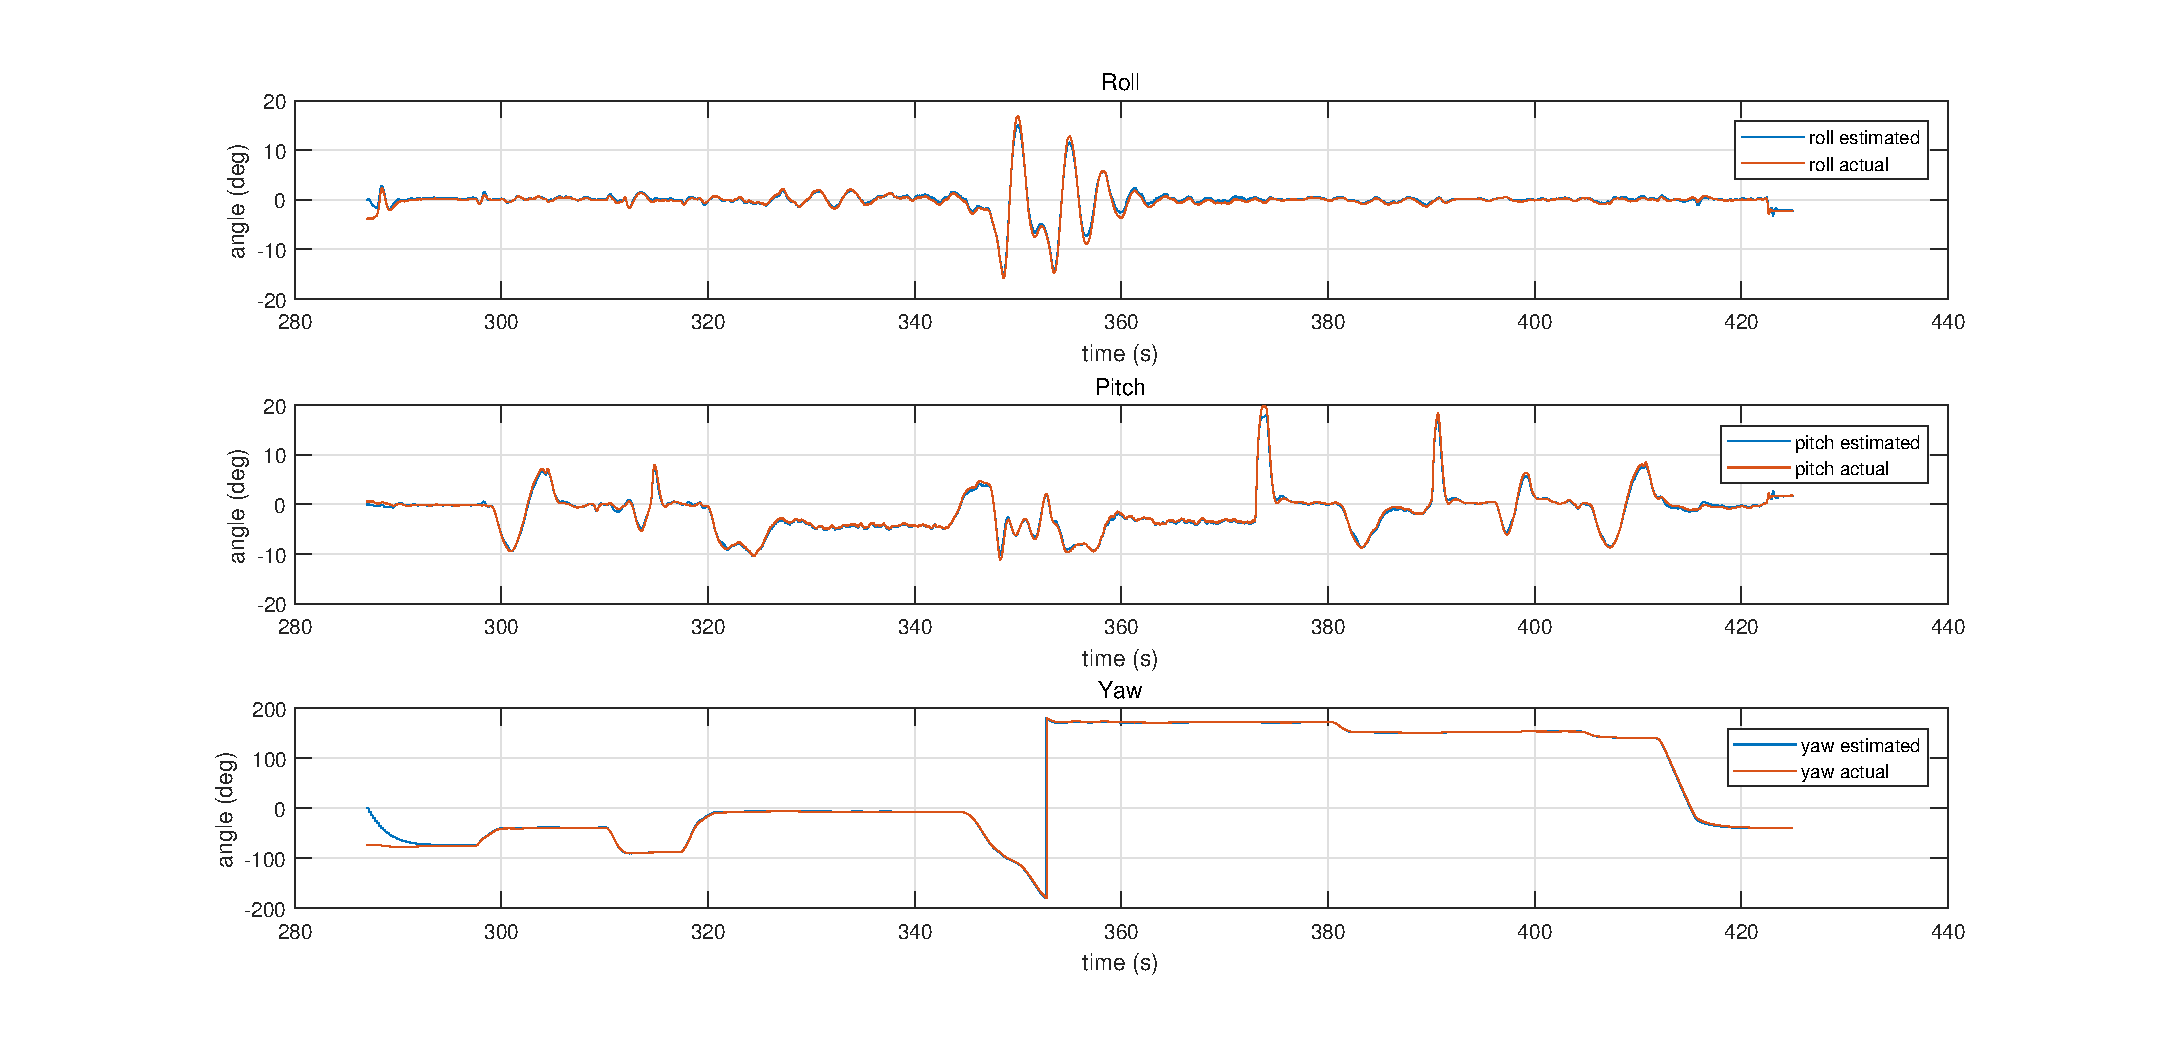
\includegraphics[width=1.0\textwidth]{attitude1.eps}
	\bicaption{姿态对比}{Attitude comparison}
	\label{fig:attitude}
\end{figure} 
从\autoref{fig:attitude}中我们看出,我们估计的姿态和原本飞控板给出的姿态基本一致,表面算法整体是收敛的。

另一方面,RTK能输出世界坐标系下的位置和速度,我们可以通过对比估计器输出的位置、速度和RTK输出的位置、速度的一致性可以评估位置融合的效果。
\autoref{fig:velocity}是速度对比图。
\begin{figure}[htbp]
	\centering
	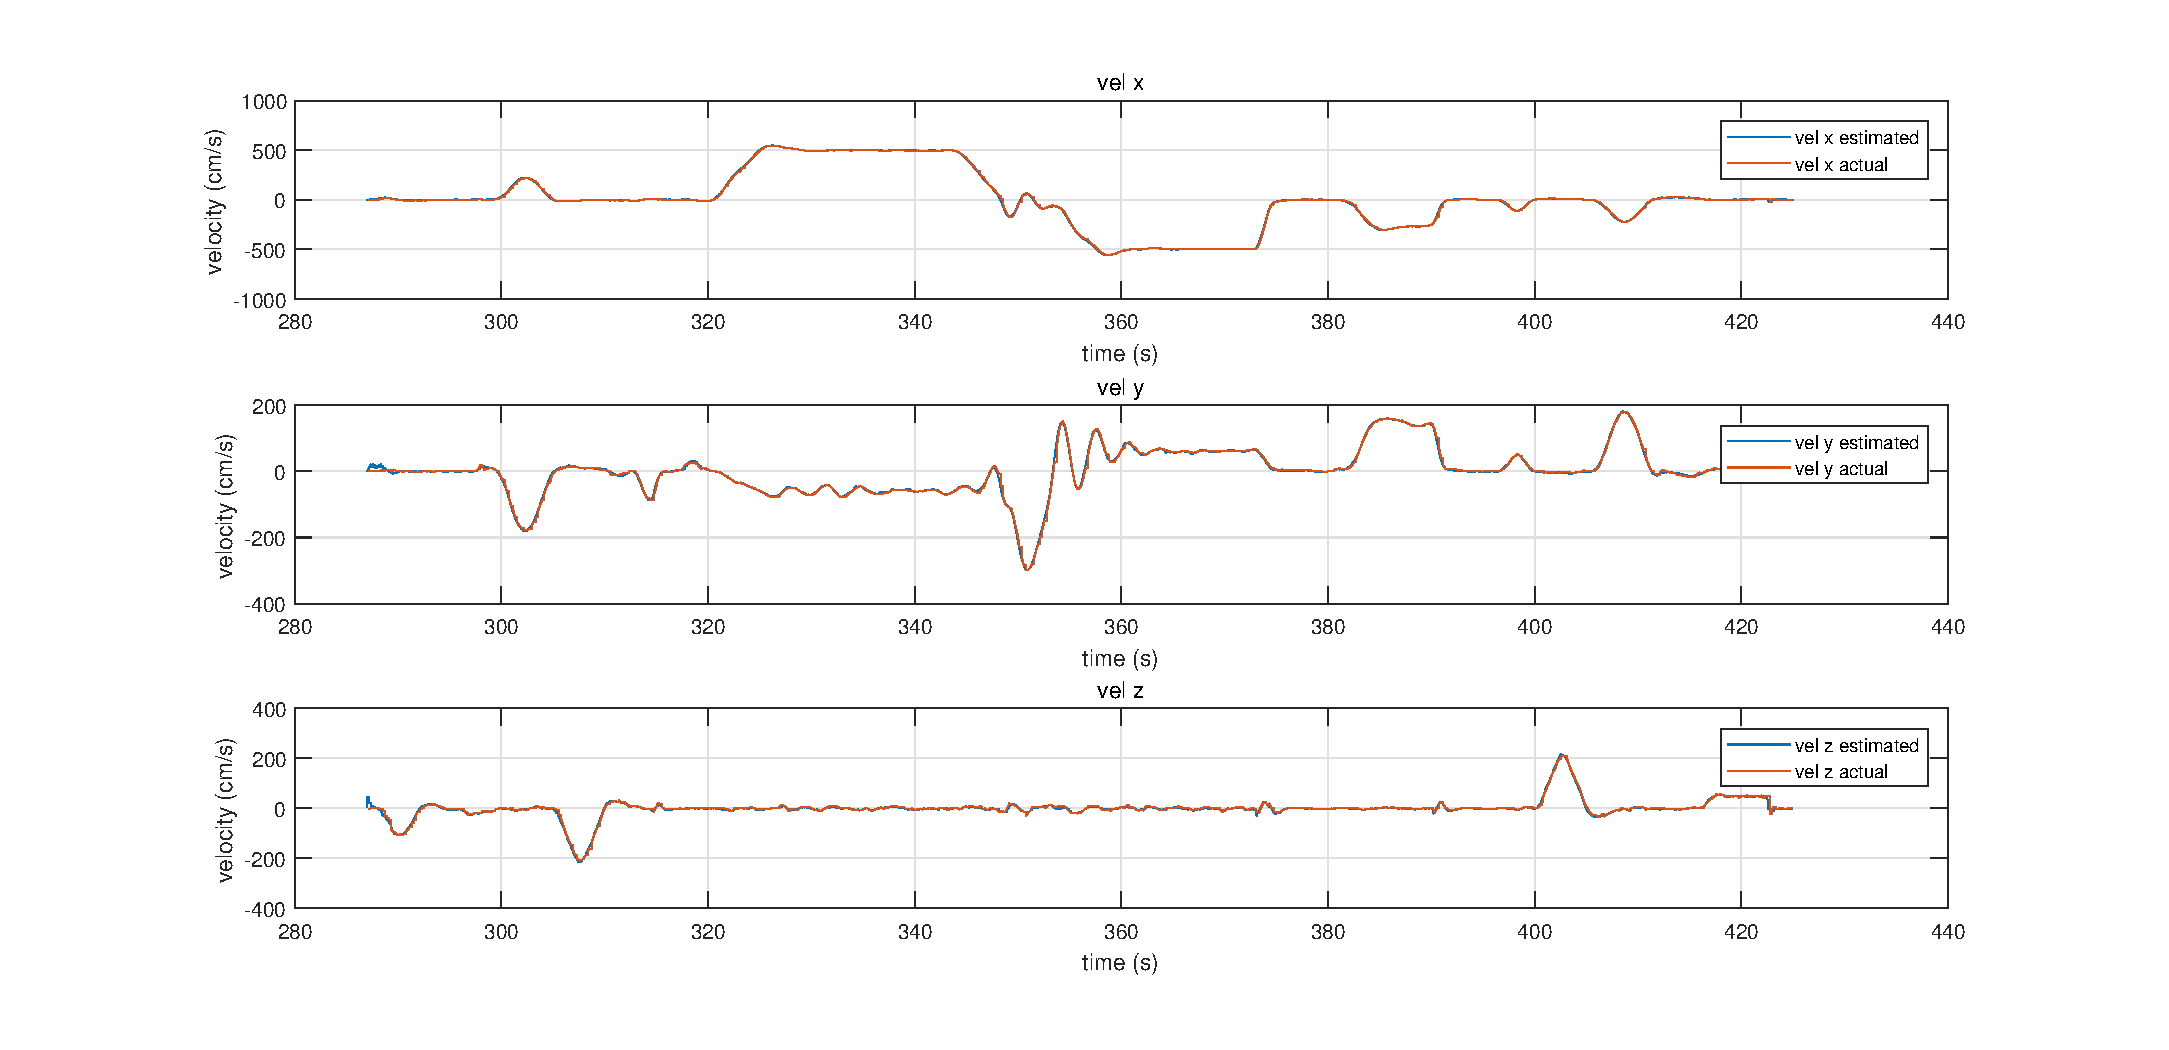
\includegraphics[width=1.0\textwidth]{velocity.eps}
	\bicaption{速度对比}{Velocity comparison}
	\label{fig:velocity}
\end{figure}

\autoref{fig:position}是位置对比图。
\begin{figure}[htbp]
	\centering
	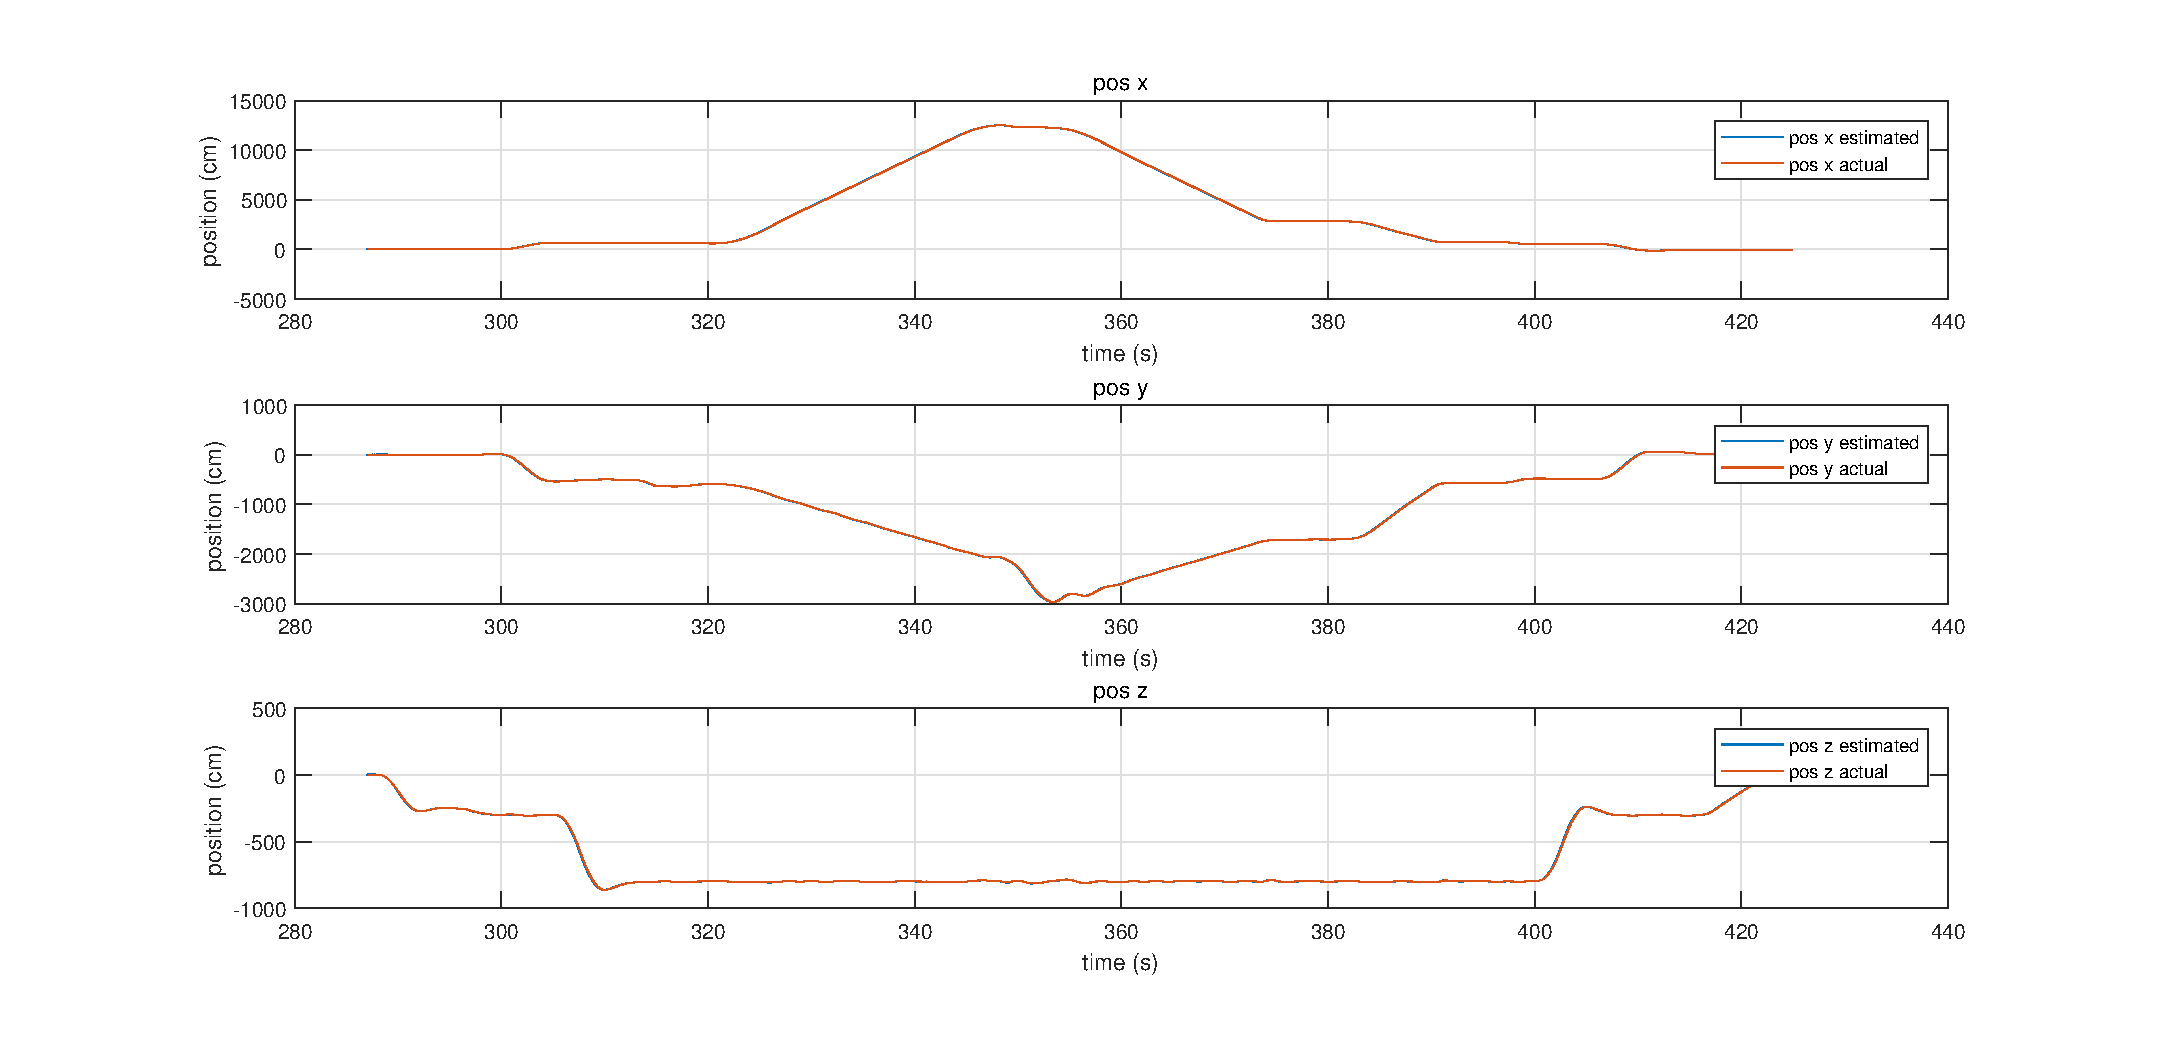
\includegraphics[width=1.0\textwidth]{position.eps}
	\bicaption{位置对比}{Position comparison}
	\label{fig:position}
\end{figure}
从\autoref{fig:velocity}以及\autoref{fig:position}中我们看出,我们估计的位置和速度和RTK输出的位置和速度基本一致,表面算法整体是收敛的。

接下来我们量化估计器的性能指标,对于姿态来说,我们使用运动加速度间接计算估计器的精确度,我们首先通过估计器输出的姿态求出估计器输出的运动加速度,然后通过RTK输出的速度差分求出RTK输出的运动加速度,通过分析二者的误差可以评估估计器的性能指标。

\autoref{fig:motionacc}是运动加速度对比图。
\begin{figure}[htbp]
	\centering
	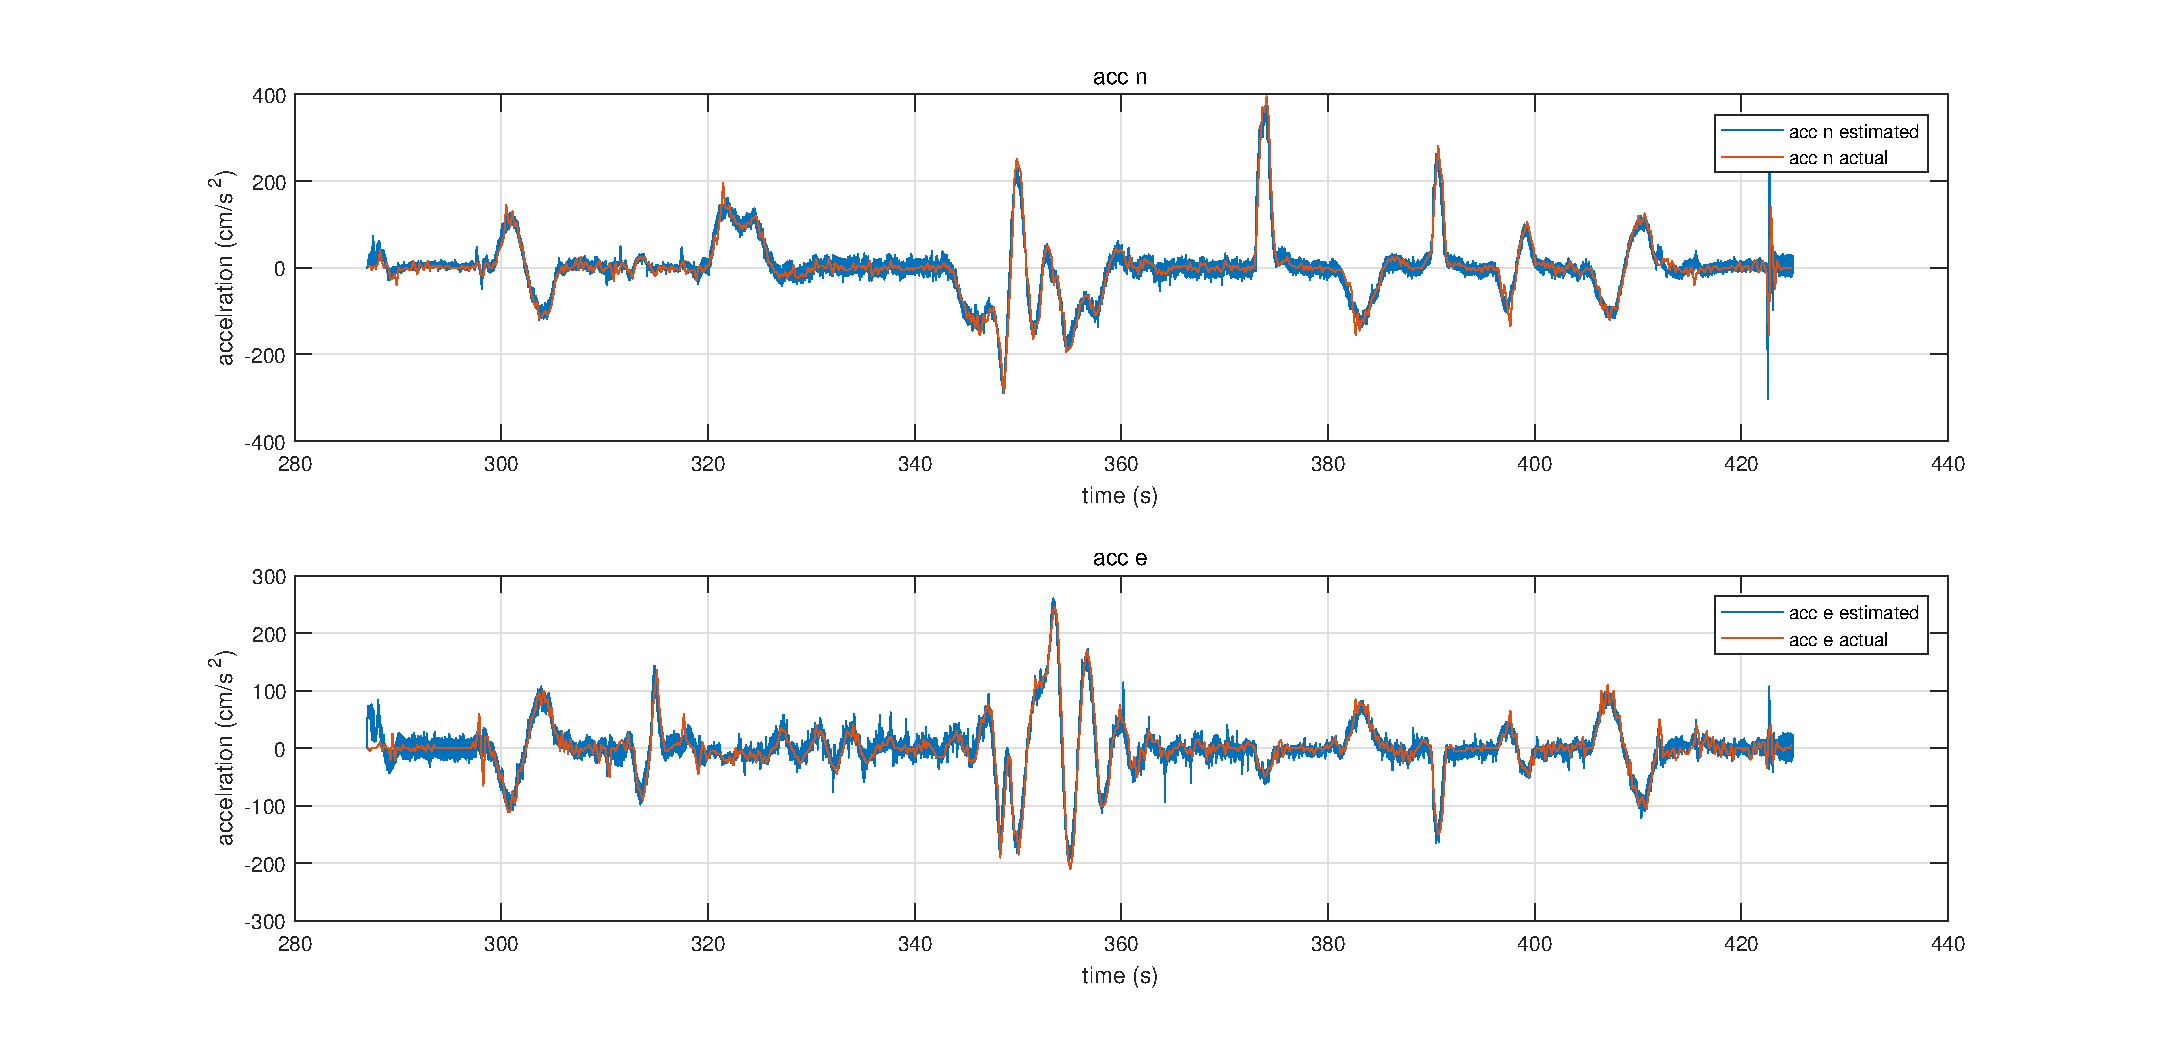
\includegraphics[width=1.0\textwidth]{motionacc.eps}
	\bicaption{运动加速度对比}{Motion acceleration comparison}
	\label{fig:motionacc}
\end{figure}
可见,二者的运动加速度基本一致。

接下来我们进行误差分析,我们给出各个状态误差的曲线图,如\autoref{fig:error}。
\begin{figure}[htbp]
	\centering
	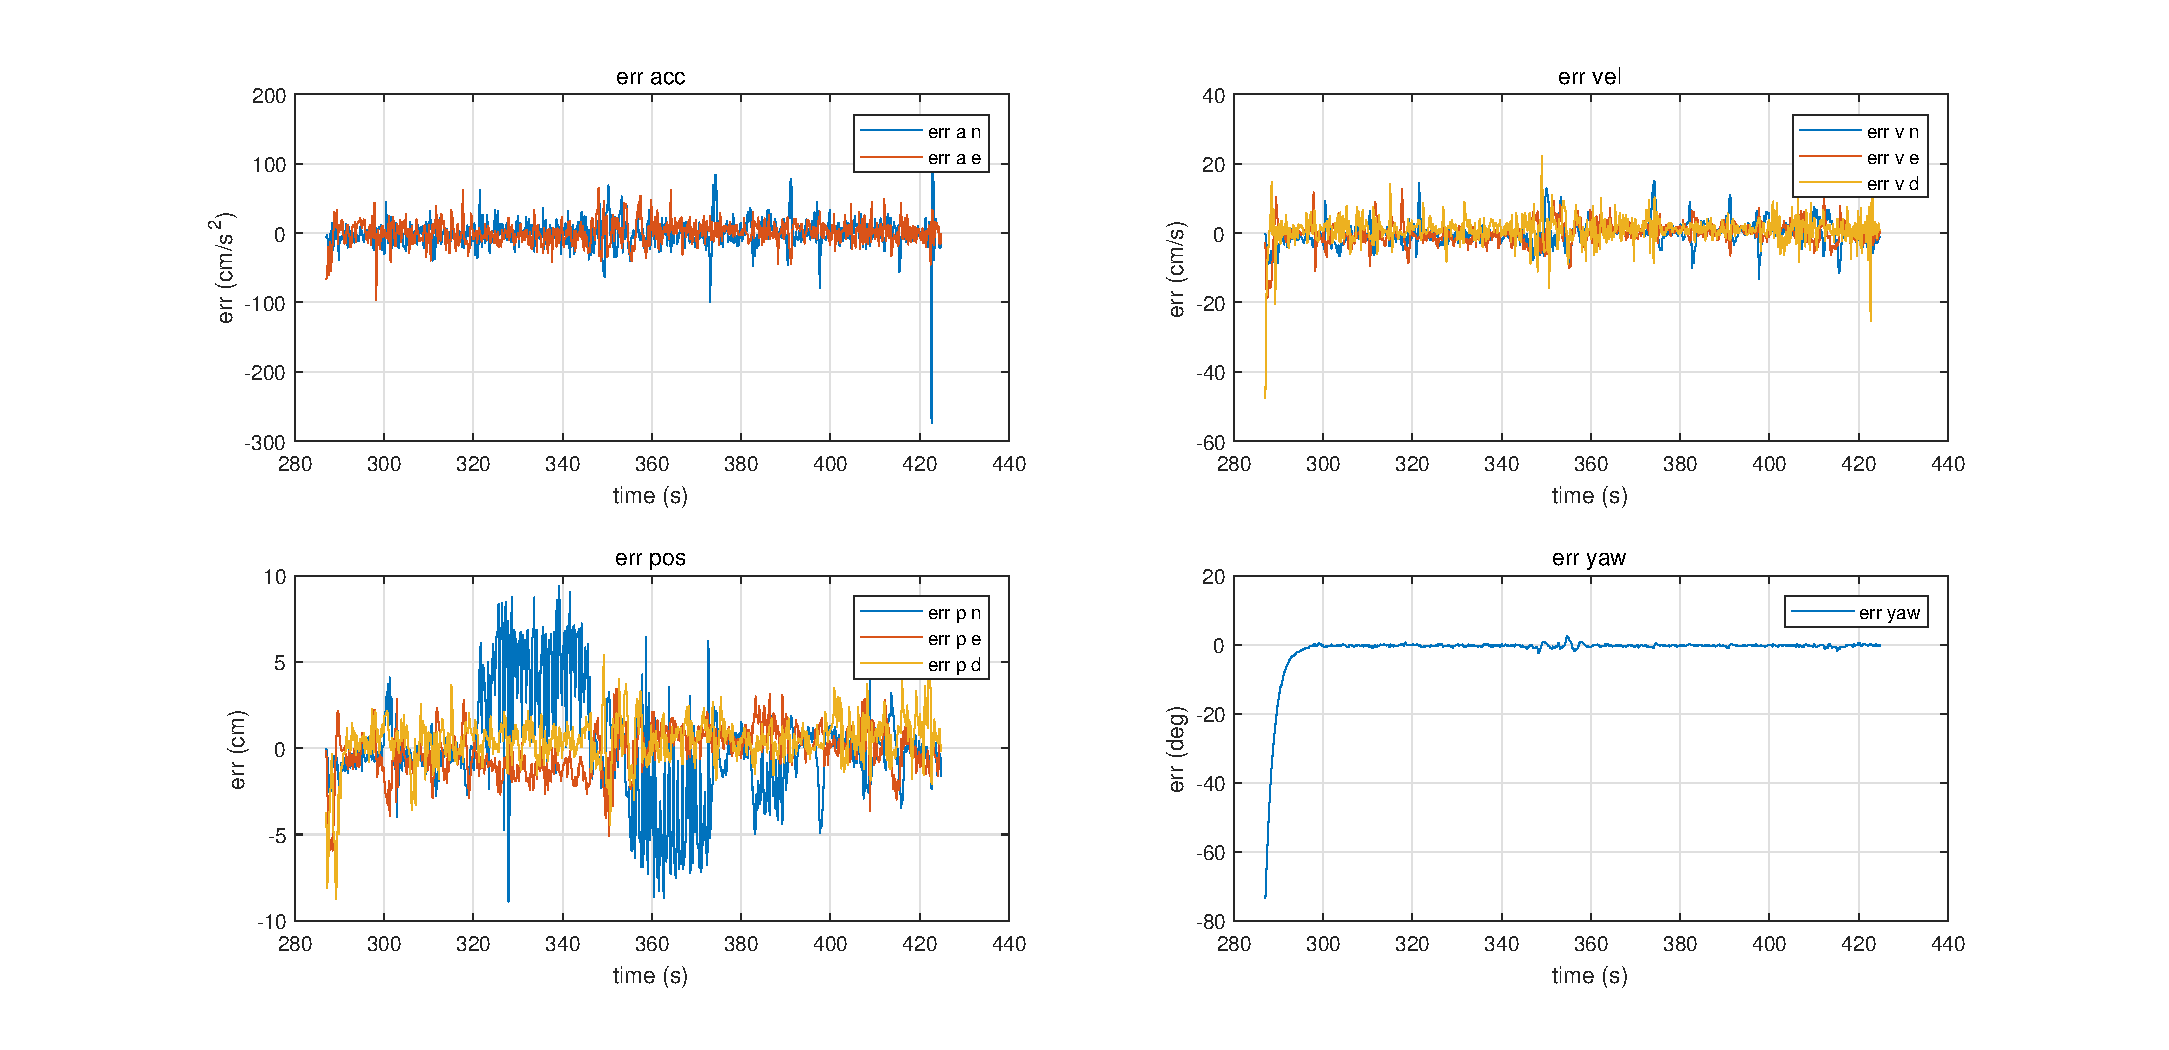
\includegraphics[width=1.0\textwidth]{error.eps}
	\bicaption{状态误差分析}{State error analysis}
	\label{fig:error}
\end{figure}
接下来我们会给出误差的标准差。

整体飞行轨迹如\autoref{fig:trajectory}所示
\begin{figure}[htbp]
	\centering
	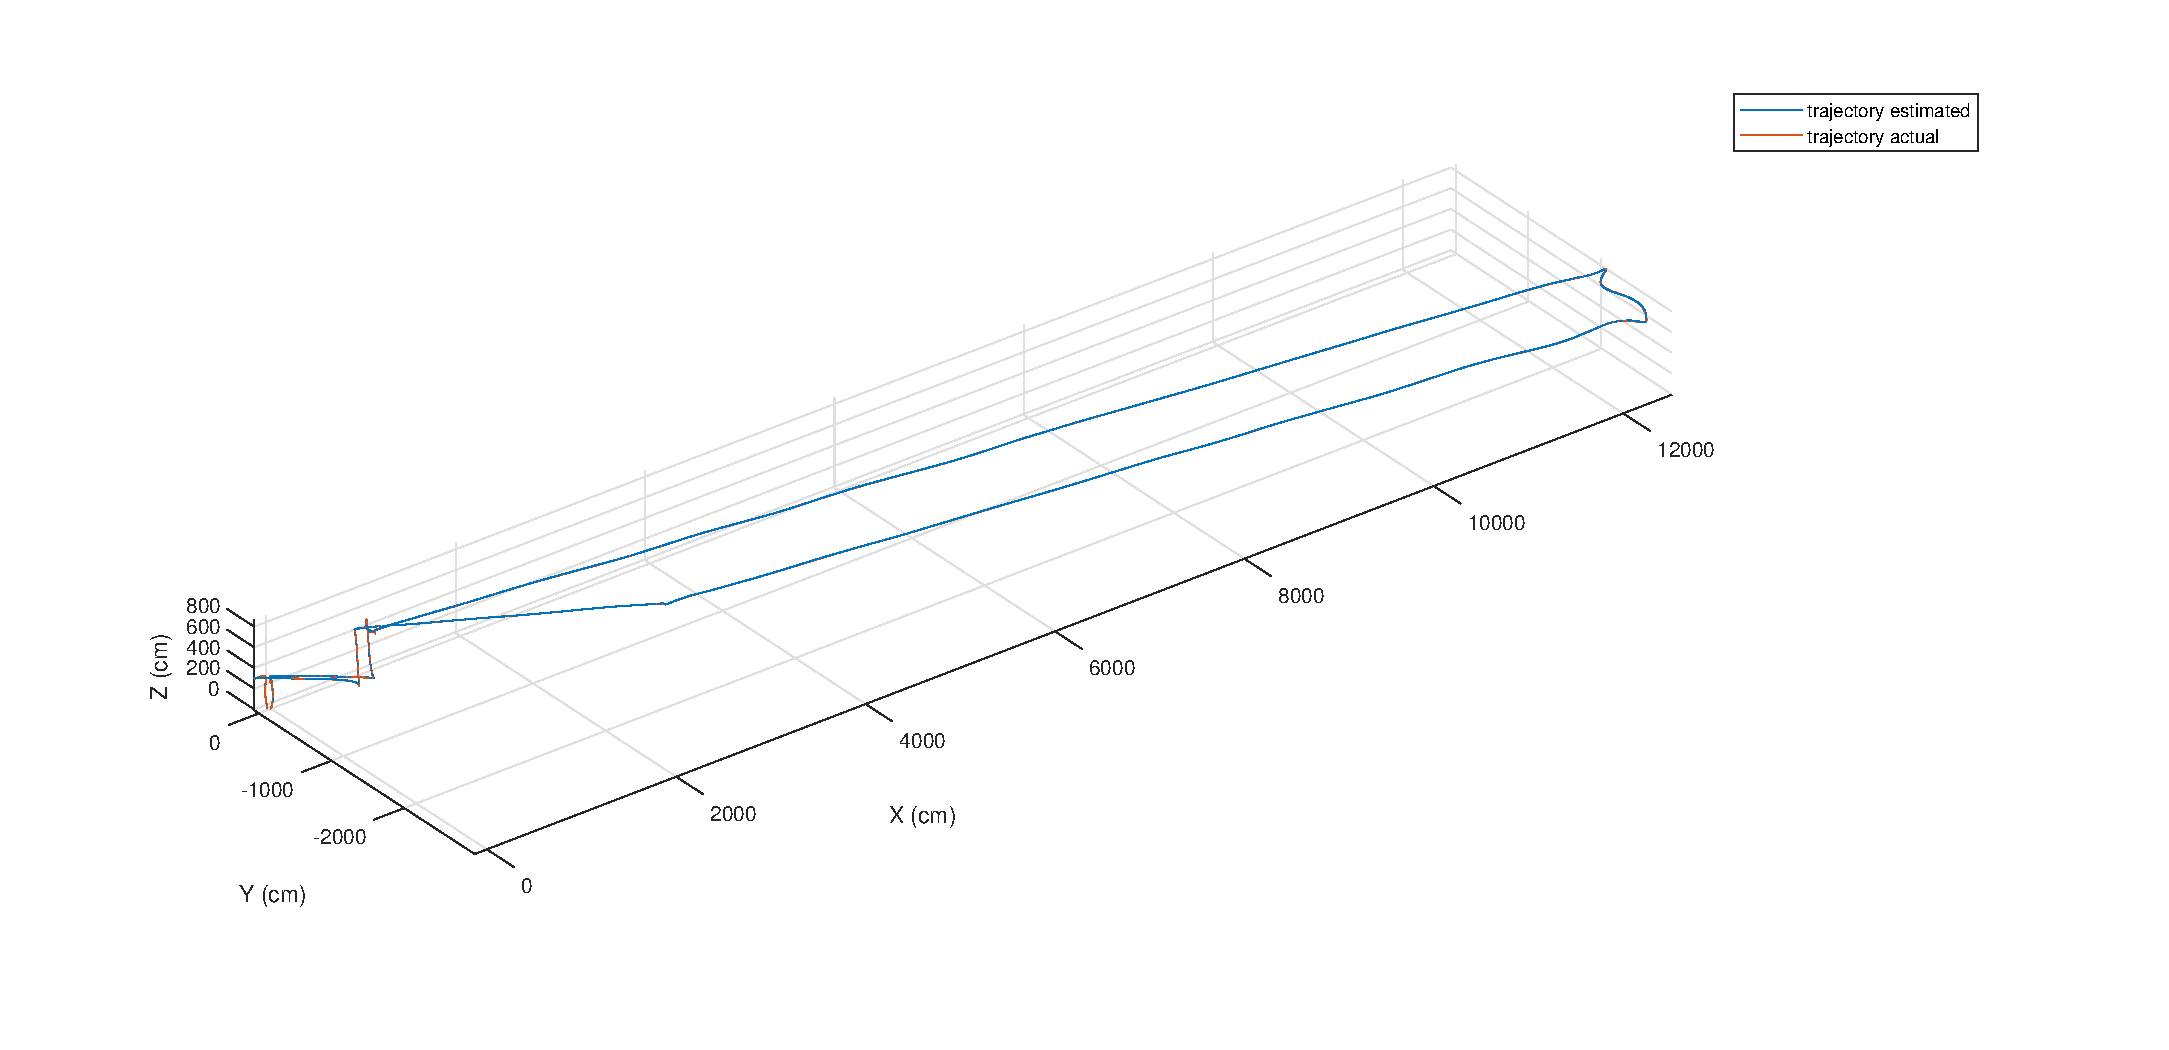
\includegraphics[width=1.0\textwidth]{trajectory.eps}
	\bicaption{飞行轨迹}{Flight trajectory}
	\label{fig:trajectory}
\end{figure}

下面,我们给出RTK和板载估计的标准差,如\autoref{stdestimate}所示。
其中,运动加速度的标准差记为$\big\{ \sigma_{a_x},\sigma_{a_y} \big\}$,
偏航角$\psi$的标准差记为$\sigma_{\psi}$,
位置的标准差记为$\big\{ \sigma_{p_x},\sigma_{p_y},\sigma_{p_z} \big\}$,
速度的标准差记为$\big\{ \sigma_{v_x},\sigma_{v_y},\sigma_{v_z} \big\}$。

\begin{table}[htbp]
	\bicaption{估计值标准差}{Standard error of estimation}
	\label{stdestimate}
	\begin{tabular}{cc}
		\toprule
		状态量 & 标准差 \\
		\midrule
		$\big\{ \sigma_{a_x},\sigma_{a_y} \big\}$ & $\big\{ 22.61, 17.28 \big\}$(cm/s) \\
		$\sigma_{\psi}$ & $6.36$(deg)   \\
		$\big\{ \sigma_{p_x},\sigma_{p_y},\sigma_{p_z} \big\}$ & $\big\{ 3.21, 1.37, 1.44 \big\}$(cm)   \\
		$\big\{ \sigma_{v_x},\sigma_{v_y},\sigma_{v_z} \big\}$ & $\big\{ 3.37, 3.31, 4.26 \big\}$(cm/s)   \\
		\bottomrule
	\end{tabular}
\end{table}

\gdutsubsection{算法对比}{Algorithm comparison}

\gdutsubsection{传感器扰动下评估估计器的性能}{Evaluate the performance of the estimator under sensor disturbance}

\gdutsection{总结与讨论}{Summary and discussion}
在本章中,我们展示了使用IMU作为主要传感器,融合其他传感器进行状态估计以实现飞行器的稳定飞行。
我们提出了预测-修正-延时融合框架,以处理多频率多延时的传感器系统。
我们对每个传感器的特性进行研究,针对磁场干扰及运动加速度补偿进行优化处理,以提高系统的鲁棒性。
本文提出的算法可以使飞行器保持稳定。

\gdutchapter{基于多位置法的IMU校准算法研究}{Research on IMU calibration algorithm based on multi-position method}
在本章中,我们研究如何使用较少的仪器来进行高精度的传感器校准以提供更好的传感器数据。
一般来说,基于MEMS的传感器的精度都比较差,远远达不到高精度导航的要求。
然而,开发基于MEMS的传感器的飞行器,要保证传感器数据精度是很困难的。
我们研究传感器校准算法,开发了一种不需要外部设备就可以进行较高精度的校准。
我们详细介绍了基于优化的传感器校准算法,并将其与融合和控制方法(第4章)结合起来进行实验,以验证系统的性能。

本系统的关键技术是一种传感器校准算法,能够无需外部设备的情况下进行校准。
我们要求校准算法能够使用人手就能完成,无需外部设备,在尽量简单的校准流程下保证校准结果的准确性。

\gdutsection{问题描述}{Problem formulation}
基于MEMS的低成本IMU误差通常包括不精确的尺度、传感器敏感轴不对齐和零偏的影响。
IMU校准指的是辨识这些物理量的过程。
我们首先要将这些参数用数学语言描述出来,以便我们综合设计算法。

\gdutsubsection{传感器误差模型}{Sensor error model}
在第二章我们已经对传感器建立了数学模型,但这个模型是校准后的模型。
下面描述的是校准前的模型。

对于一个理想的IMU,三轴传感器应该具备相同的三维正交敏感轴,比例因子应该将每个传感器测量的数字量转换为真实的物理量(如加速度和角速度)。
实际上,基于MEMS的低成本IMU误差通常包括不精确的尺度、传感器敏感轴不对齐和零偏的影响。

轴正交误差可以建模成一个矩阵
\begin{equation}\label{eq:axiserror}
	T=
	\begin{bmatrix}
		1 & \beta_{yz} & \beta_{zy}\\
		\beta_{xz} & 1 & \beta_{zx}\\
		\beta_{xy} & \beta_{yx} & 1
	\end{bmatrix}
\end{equation}
其中,$T$是轴正交矩阵,$\beta_{ij}$是第$i$个传感器轴的误差对第$j$个轴的造成的误差影响。

比例因子误差可以建模成一个对角阵
\begin{equation}\label{eq:scaleerror}
	K=
	\begin{bmatrix}
		s_x & 0 & 0\\
		0 & s_y & 0\\
		0 & 0 & s_z
	\end{bmatrix}
\end{equation}
零偏可以建模成一个向量
\begin{equation}\label{eq:scaleerror}
	b=
	\begin{bmatrix}
		b_x\\
		b_y\\
		b_z
	\end{bmatrix}
\end{equation}
完整的传感器误差模型为
\begin{equation}\label{eq:sensorerrormodel}
	x^O=T K (x^S + b + \nu)
\end{equation}
其中,$x$指一种三轴传感器,$x^O$和$x^S$分别表示校准后和校准前的传感器数据,$ν$是传感器测量噪声。
那么我们可以由\autoref{eq:sensorerrormodel}写出加速度计和陀螺仪的误差模型。

加速度计的误差模型为
\begin{equation}
	a^O=T^a K^a (a^S + b^a + \nu^a)
\end{equation}
陀螺仪的误差模型为
\begin{equation}\label{eq:accerrormodel}
	\omega^O=T^\omega K^\omega (\omega^S + b^\omega + \nu^\omega)
\end{equation}
从而,我们也得到需要求解的参数,将这些参数定义为
\begin{equation}\label{eq:thetadef}
	\theta = 
	\begin{bmatrix}
		\beta_{yz},\beta_{zy},\beta_{xz},\beta_{zx},\beta_{xy}, \beta_{yx},s_x,s_y,s_z,b_x,b_y,b_z
	\end{bmatrix}
\end{equation}
那么我们可以由\autoref{eq:thetadef}写出加速度计和陀螺仪的待求参数。

加速度计的待求参数向量为
\begin{equation}
	\theta^a = 
	\begin{bmatrix}
		\beta_{yz}^a,\beta_{zy}^a,\beta_{xz}^a,\beta_{zx}^a,\beta_{xy}^a, \beta_{yx}^a,s_x^a,s_y^a,s_z^a,b_x^a,b_y^a,b_z^a
	\end{bmatrix}
\end{equation}
陀螺仪的待求参数向量为
\begin{equation}
	\theta^\omega = 
	\begin{bmatrix}
		\beta_{yz}^\omega,\beta_{zy}^\omega,\beta_{xz}^\omega,\beta_{zx}^\omega,\beta_{xy}^\omega, \beta_{yx}^\omega,s_x^\omega,s_y^\omega,s_z^\omega,b_x^\omega,b_y^\omega,b_z^\omega
	\end{bmatrix}
\end{equation}

\gdutsection{校准算法分析}{Calibration algorithm analysis}
将校准问题用数学语言表述之后,我们将讨论具体的算法实现,分析各种算法的优劣以及目前存在的问题,以引出我们的设计。

\gdutsubsection{外部设备}{External equipments}
IMU校准的传统方法是通过使用特殊的机械平台来完成的,如机器人机械手、转台。
具体操作是以已知的旋转速度移动IMU到精确控制的姿态上\cite{hall2000case}。
在每个姿态上,加速度计的输出与预先计算的重力向量进行比较,而在旋转期间,陀螺仪的输出与预先计算的旋转速度进行比较。
然而,用于校准的机械平台通常非常昂贵,导致校准成本往往超过IMU的硬件成本。

\gdutsubsection{多位置法}{Multi-position method}
多位置法最早是由Lotters等人提出的\cite{lotters1998procedure}。
Lotters等人提出,利用静态加速度的大小必须等于重力的大小这一事实,来校准加速度计的零偏和尺度。
所有参数都可以通过在一组静态姿态上最小化残差来估计。
在校准完加速度计后,可以利用加速度计测量到的重力矢量位置作为基准来校准陀螺仪。
积分两个连续静止位置之间的角速度,可以估计在新位置上的重力向量。
最终通过这些估计值与校准后的加速度计给出的重力参考值之间的误差最小化来校准陀螺仪。
此方法适用于底成本IMU校准上。

\gdutsection{基于多位置法的IMU校准}{Multi-position method based IMU calibration}
本节描述了一种校准IMU的方法,以提高IMU本身的数据精度。
这项工作的主要目标是开发一种无需外部设备,只需要用手移动传感器,并将其置于一组不同的静态位置(姿态),通过简单的流程就能实现校准。
我们的关键贡献是一种基于\cite{tedaldi2014robust}的方法,提出了新的最优阈值的算法,改进了参数估计算法,提高了IMU本身输出数据的精度。
\begin{figure}[htbp]
	\centering
	\includegraphics[width=0.3\textwidth]{屏幕截图 2022-04-03 100222.png}
	\bicaption{校准流程图}{Flow chart of calibration}
	\label{fig:Flowchartofcalibration}
\end{figure}

\gdutsubsection{校准流程}{Calibration procedure}
如上一节所介绍的,本文的校准流程需要收集原始加速度计和陀螺仪读数的数据集,当操作员将IMU移动到不同的静态位置时,产生了一组明显的、稳定的旋转。
我们的IMU校准流程如\autoref{fig:Flowchartofcalibration}。
\autoref{fig:Flowchartofcalibration}中的$t_wait$是每个静态区间的最大长度。
\autoref{fig:Flowchartofcalibration}中的$T_{init}$是初始化静止时间,初始化阶段是用于计算陀螺仪零偏和静态检测系数。
我们记校准流程中IMU旋转的姿态次数为N。
为了避免校准参数估计中的不可观性,至少需要收集12组不同姿态的。
一般来说,N越大,校准结果越好。
同时保持每个静态间隔的持续时间减少,以满足陀螺仪零偏不变的假设。
参数估计算法后面给出伪代码。

\gdutsubsection{非线性优化}{Nonlinear optimization}
我们使用非线性优化的方法估计IMU参数。
首先需要写出加速度计和陀螺仪的代价函数。

我们定义以下函数:
\begin{equation}
	a^O=h(a^S,\theta^a) =T^a K^a (a^S + b^a)
\end{equation}
这里,我们可以忽略测量噪声,这是因为在我们的校准程序中,我们对每个静态区间的加速度信号求均值。
我们记录N组稳定的姿态。
我们在每个静态间隔内的一个时间窗口内平均加速度计读数可以提取M个加速度矢量$a^S_k$。
我们用来估计加速度计参数的代价函数为:
\begin{equation}\label{eq:costacc}
	L(\theta^a)=\sum_{k=1}^{M}(\left\|g\right\|-\left\|h(a^S,\theta^a)\right\|)^2
\end{equation}
其中,$\left\|g\right\|$是当地重力矢量的实际大小。
为了使\autoref{eq:costacc}最小化,我们使用Levenberg-Marquardt(LM)算法。

为了校准陀螺仪,我们可以假设陀螺仪是无偏的。
此外,由于我们需要使用加速度计作为已知参考,因此我们使用上面计算的校准参数$\theta^a$,用\autoref{eq:accerrormodel}对加速度计读数进行校准。

我们有陀螺仪数据可以在一段时间内积分出旋转,可以计算出结束位置的重力矢量。
函数定义如下:
\begin{equation}\label{eq:integration}
	u_{g,k}=\phi(\omega^S_i , u_{a,k-1})
\end{equation}
其中,$\omega^S_i$是n个陀螺仪读数的序列,$u_{a,k-1}$是一个初始重力矢量,$u_{g,k}$是终点重力矢量,$\phi$是通过积分输入角速度来计算最终位置的积分算法。
在这种情况下,我们可以定义代价函数为:
\begin{equation}\label{eq:costgyro}
	L(\theta^\omega)=\sum_{k=2}^{M}(u_{a,k}-u_{g,k})^2
\end{equation}
同理,我们使用LM算法最小化\autoref{eq:costgyro}求解$\theta^\omega$。

\gdutsubsection{静态检测}{Static detector}
校准的精度在很大程度上取决于静态和运动区间的可靠性:
加速度计的校准采用静态区间,而陀螺仪的校准也采用两个连续静态区间之间的运动区间。
基于带通滤波器的算法,比如\cite{fong2008methods}中使用的准静态检测器,在实际数据集上表现很差:
检测到的静态区间经常包含一小部分运动。
此外,它们还需要进行微调,因为算法依赖于三个参数。
我们的检测器基于基于Tedaldi的方法\cite{tedaldi2014robust}:对于每个加速度计样本$\begin{bmatrix}
	a^t_x & a^t_y & a^t_z
\end{bmatrix}$,给定一个长度为$t_{wait}$秒的时间间隔时刻,我们计算方差的大小
\begin{equation}\label{eq:var}
	\zeta(t)=\sqrt{[var_{t_w}(a^t_x)]^2+[var_{t_w}(a^t_y)]^2+[var_{t_w}(a^t_z)]^2}
\end{equation}
其中$var_{t_w}(a^t)$是一个运算符,计算加速度计$a^t$在以$t$为中心,长度为$t_w$秒的时间间隔内的方差。
我们通过判断$\zeta(t)$是否小于或大于一个阈值对静态和运动间隔进行分割。
作为阈值,我们考虑方差大小平方$\zeta_{init}$的整数倍。
其中,$\zeta_{init}$是初始化阶段的方差。
需要注意的是,Tedaldi的静态检测器不需要任何参数调整:
检测中使用的系数由Tedaldi的校准算法自动估计(参见第IV-D节)。
而我们将提出一种新的系数估计算法。
\autoref{fig:staticdetection}显示了静态检测是如何处理真实数据的。
\begin{figure}[htbp]
	\centering
	\includegraphics[width=0.7\textwidth]{屏幕截图 2022-04-03 103640.png}
	\bicaption{静态检测示意图}{Diagram of static detection}
	\label{fig:staticdetection}
\end{figure}
静态检测器由黑色方波表示,它的高电平是一个静态区间。

\gdutsubsection{龙格-库塔积分}{Runge-Kutta Integration}
如\autoref{eq:integration}所述,在陀螺仪校准中,我们需要对离散时间角速度进行积分。
因此需要一种鲁棒且稳定的数值积分方法以提高校准精度。
由于我们使用四元数算法表示旋转,在此描述下,合适的积分算法选择是四阶龙格-库塔法(RK4n)\cite{andrle2013geometric}。
RK4n优于标准的线性积分算法,输出更高精度的结果。
定义四元数运动学的微分方程如下:
\begin{equation}
	\dot{q}(k)=f(\cdot )=\frac{1}{2} q \otimes \mathbf{p}(\omega_y(k))
\end{equation}
RK4n积分算法如下:
\begin{equation}\label{eq:rk4}
	\begin{aligned}
		q_{k+1} &= q_k + \frac{\Delta t}{6}(k_1 + 2 k_2 + 2 k_3 + k_4)\\
		k_1 &= f(t_k , q_k)\\
		k_2 &= f(t_k + \frac{\Delta t}{2},q_k + \frac{\Delta t}{2} k_1)\\
		k_3 &= f(t_k + \frac{\Delta t}{2},q_k + \frac{\Delta t}{2} k_2)\\
		k_4 &= f(t_k + \Delta t, q_k + \Delta t k_3)\\
	\end{aligned}
\end{equation}
最后,对于每一步,我们还需要对k+1时刻四元数进行归一化:
\begin{equation}
	q_{k+1} = \frac{q_{k+1}}{\left\|q_{k+1}\right\|}
\end{equation}

\gdutsubsection{IMU参数估计算法}{IMU parameter estimation algorithm}
我们前面介绍了非线性优化、静态检测以及龙格库塔积分算法,接下来我们将他们组合起来形成我们最后的参数估计算法。
我们首先通过校准流程采集到加速度计和陀螺仪的数据集。
然后在初始化阶段可以算出陀螺仪的零偏$b^\omega$以及通过\autoref{eq:var}计算$\zeta_{init}$。

根据Tedaldi的算法\cite{tedaldi2014robust},通过$\zeta_{init}$的整数倍设置阈值,检测静态区间,最小化\autoref{eq:costacc},根据残差和的大小来选取最优的阈值。
但从原理上,残差和其实与样本数量也有关系,不仅和校准的效果有关,因此采用残差和作为标准选择最优k值并不合适。
我们提出基于加速度计的静态误差作为衡量标准,计算最优k值。
静态误差定义为加速度数据与重力做差的模的均值。

选取最优k值之后,再次最小化\autoref{eq:costacc},得出加速度计的校准参数,然后通过\autoref{eq:accerrormodel}得出加速度的参考值作为陀螺仪校准的参考,最后通过最小化\autoref{eq:costgyro},求出陀螺仪的参数。
我们给出了以上算法的伪代码。

\begin{algorithm} 
	\caption{IMU Calibration} 
	\label{alg1} 
	\begin{algorithmic}
		\REQUIRE $T_{init}$ , $t_{wait}$ ; $a^S$ and $\omega^S$ (accelerometer's and
		gyroscope's dataset).
%		\rule[0.25\baselineskip]{\textwidth}{0.5pt} 
		\STATE $b^{\omega} \gets$ average gyroscope signals over $T_{init}$; 
		\STATE $\omega^S_{biasfree} \gets \omega^S - b^{\omega}$; 
		\STATE $M_{init} \gets$ empty matrix; 
		\STATE $\zeta_{init} \gets $ Eq. 14, with $t_w = T_{init}$;
		\FOR{$i=1$ \TO $k$}
		\STATE $threshold \gets i*\zeta_{init}$;
		\STATE $intervals \gets$ static detector computed using $t_{wait}$ and $threshold$;
		\STATE $Params_{acc} \gets$ optimize Eq. 11 using
		$intervals$ and $a_S$, averaging with $t_{wait}$; 
		\STATE $error \gets $ static error computed using $Params_{acc}$ and $a_S$;
		\STATE $M_{init} \gets [Params_{acc},threshold,intervals,error]$;
		\ENDFOR
		\STATE $index_{opt} \gets $ index of the minimum error in $M_{inf}$; 
		\STATE $Params_{acc} \gets $ from $M_{inf}$ using $index_{opt}$; 
		\STATE $intervals_{opt} \gets $ from $M_{inf}$ using $index_{opt}$; 
		\STATE $a^O \gets$ calibrate $a^S$ using $Params_{acc}$;
		\STATE $Params_{gyro} \gets $ optimize Eq. 13 using $intervals_{opt},\omega^S_{biasfree}$ and $a^O$, averaging with $t_{wait}$. 
	\end{algorithmic} 
\end{algorithm}

\gdutsection{实验结果}{Experimental results}
我们给出了两个实验:
(1)研究校准算法本身的性能;
(2)与标准的Tedaldi算法对比;
在第一章有说明,我们使用飞控板上的IMU作为实验平台。
IMU是BMI088。

\gdutsubsection{评估校准结果}{Evaluating calibration result}
我们按照校准流程采集IMU数据,如\autoref{fig:Flowchartofcalibration}。
接着我们执行IMU参数估计算法,静态检测效果如\autoref{fig:staticdetect}
\begin{figure}[htbp]
	\centering
	\includegraphics[width=1.0\textwidth]{staticdetect.eps}
	\bicaption{静态区间分割效果}{Static interval extraction result}
	\label{fig:staticdetect}
\end{figure}
\autoref{fig:staticdetect}是分割的可视化效果。
紫色高电平区间内为静态区间。
可见, 我们的静态检测可以取得较不错的效果。

加速度计和陀螺仪校准结果在\autoref{IMUparameters}
\begin{table}[htbp]
	\bicaption{IMU参数}{IMU parameters}
	\label{IMUparameters}
	\begin{tabular}{ccc}
		\toprule
		参数 & 加速度计 & 陀螺仪 \\
		\midrule
		$\beta_{yz}$ & -0.0039 & 0.0034\\
		$\beta_{zy}$ & 0.0081 & 0.0038\\
		$\beta_{xz}$ & 0.0002 & -0.0013\\
		$\beta_{zx}$ & -0.0037 & 0.0040\\
		$\beta_{xy}$ & -0.0072 & -0.0078\\
		$\beta_{yx}$ & 0.0047 & 0.0023\\
		$s_x$ & 0.9921 & 1.0006\\
		$s_y$ & 0.9963 & 1.0003\\
		$s_z$ & 0.9959 & 0.9993\\
		$b_x$ & 14.7897 & 2.0444\\
		$b_y$ & -7.4082 & -2.6646\\
		$b_z$ & 3.0406 & 0.5780\\
		\bottomrule
	\end{tabular}
\end{table}
在得到IMU参数后,我们对校准效果进行评估。
对于加速度计,我们观察校准前和校准后加速度的输出。
从\autoref{fig:acccalib}可以明显看出校准后的加速度更接近于重力。
\begin{figure}[htbp]
	\centering
	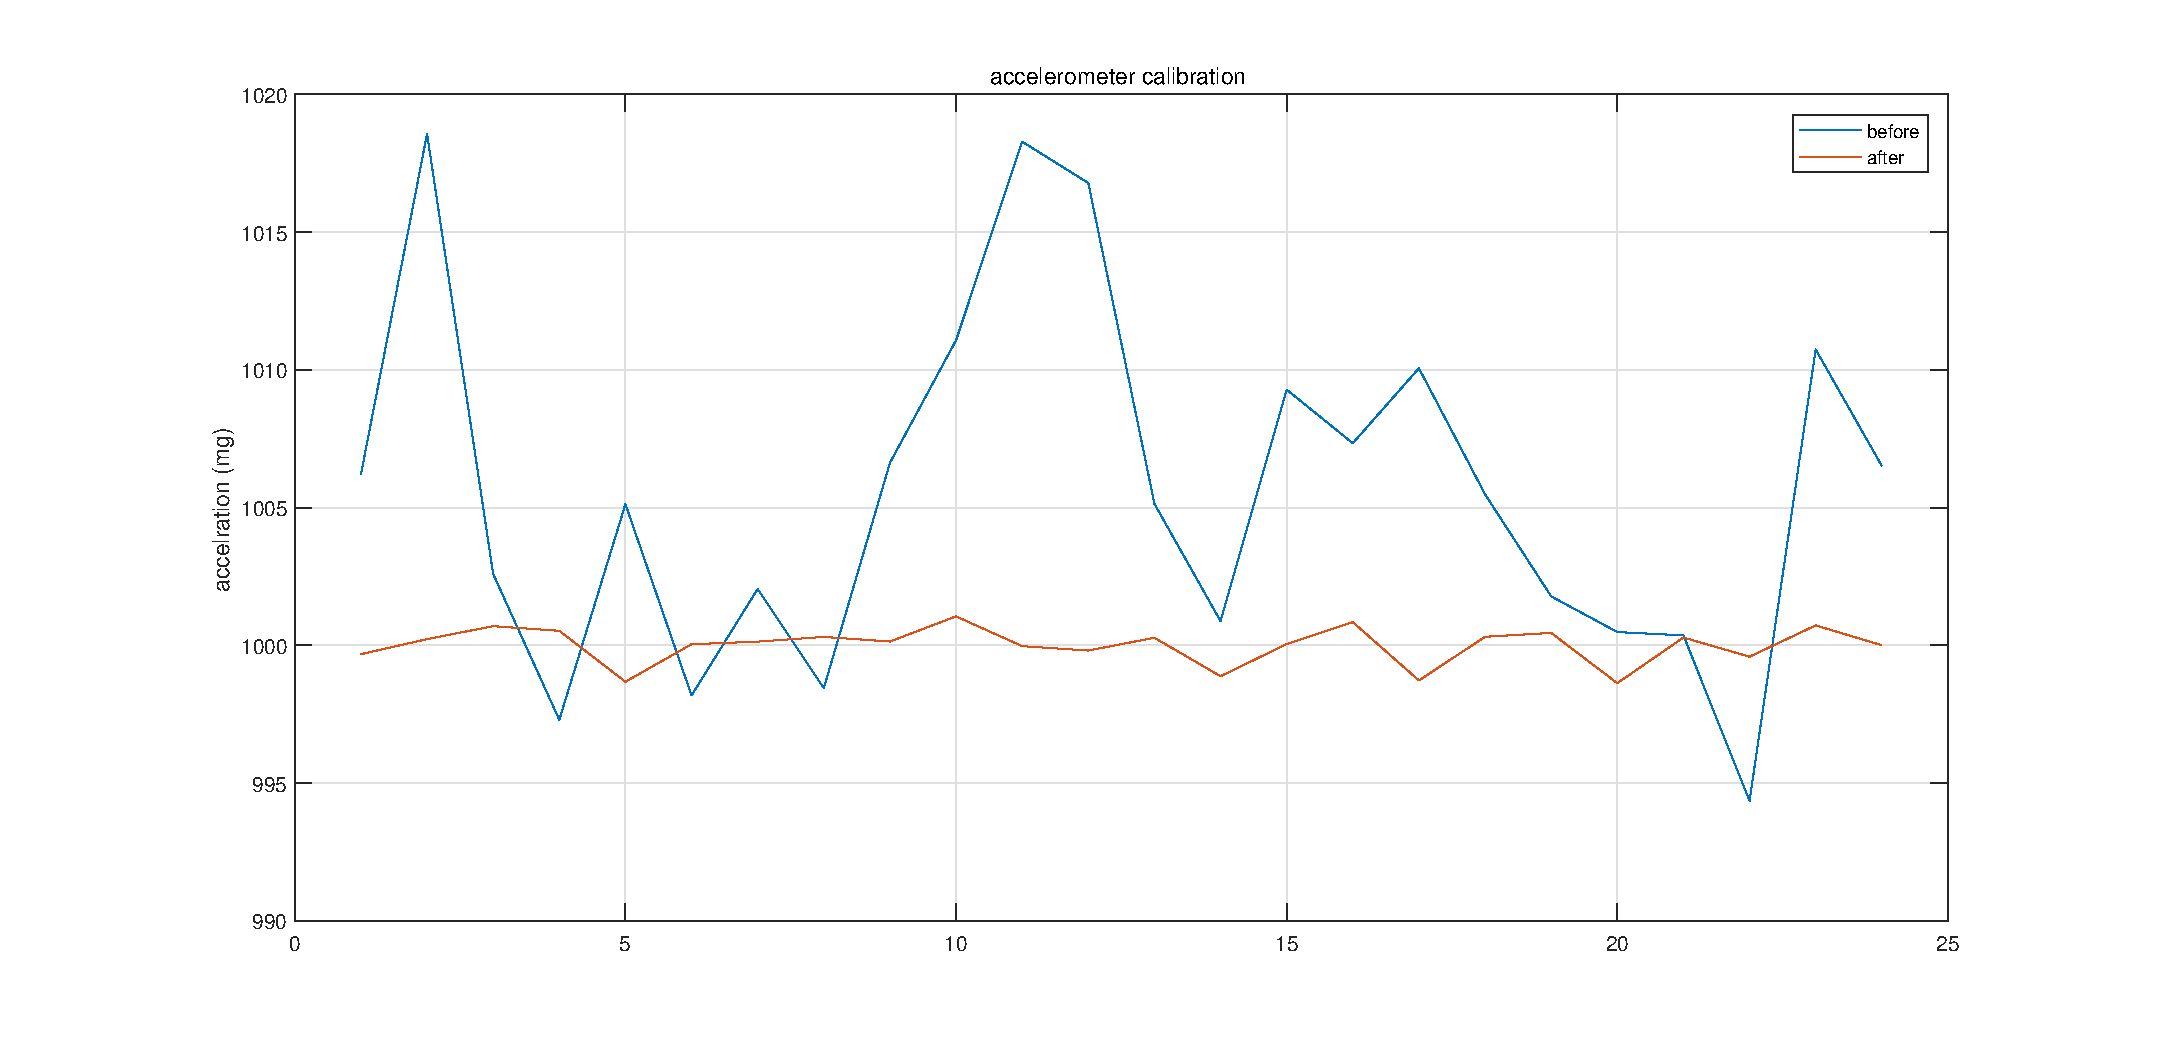
\includegraphics[width=1.0\textwidth]{acccalib.eps}
	\bicaption{加速度校准前后对比}{Acceleration calibration before and after comparison}
	\label{fig:acccalib}
\end{figure}
我们给出加速度计校准的误差分析,如\autoref{acccaliberr}
\begin{table}[htbp]
	\bicaption{加速度计校准误差}{Accelerometer calibration error}
	\label{acccaliberr}
	\begin{tabular}{ccc}
		\toprule
		状态 & 平均误差$m/s^2$ & 最大误差$m/s^2$ \\
		\midrule
		校准前 & 0.064126 & 0.181936 \\
		校准后 & 0.004935 & 0.013467 \\
		\bottomrule
	\end{tabular}
\end{table}
其中,平均误差是指加速度计输出的数据模长与重力的差的平均值,最大误差是指所有加速度计输出的数据模长中与重力的差的最大值。

对于陀螺仪,我们通过对角速度积分的姿态进行评估。
我们使用校准后的加速度计的输出作为真值。
我们进行了两个评估实验:
(1)分段区间积分对比姿态;
(2)全过程积分对比姿态;

第一个实验结果如\autoref{fig:piece}
\begin{figure}[htbp]
	\centering
	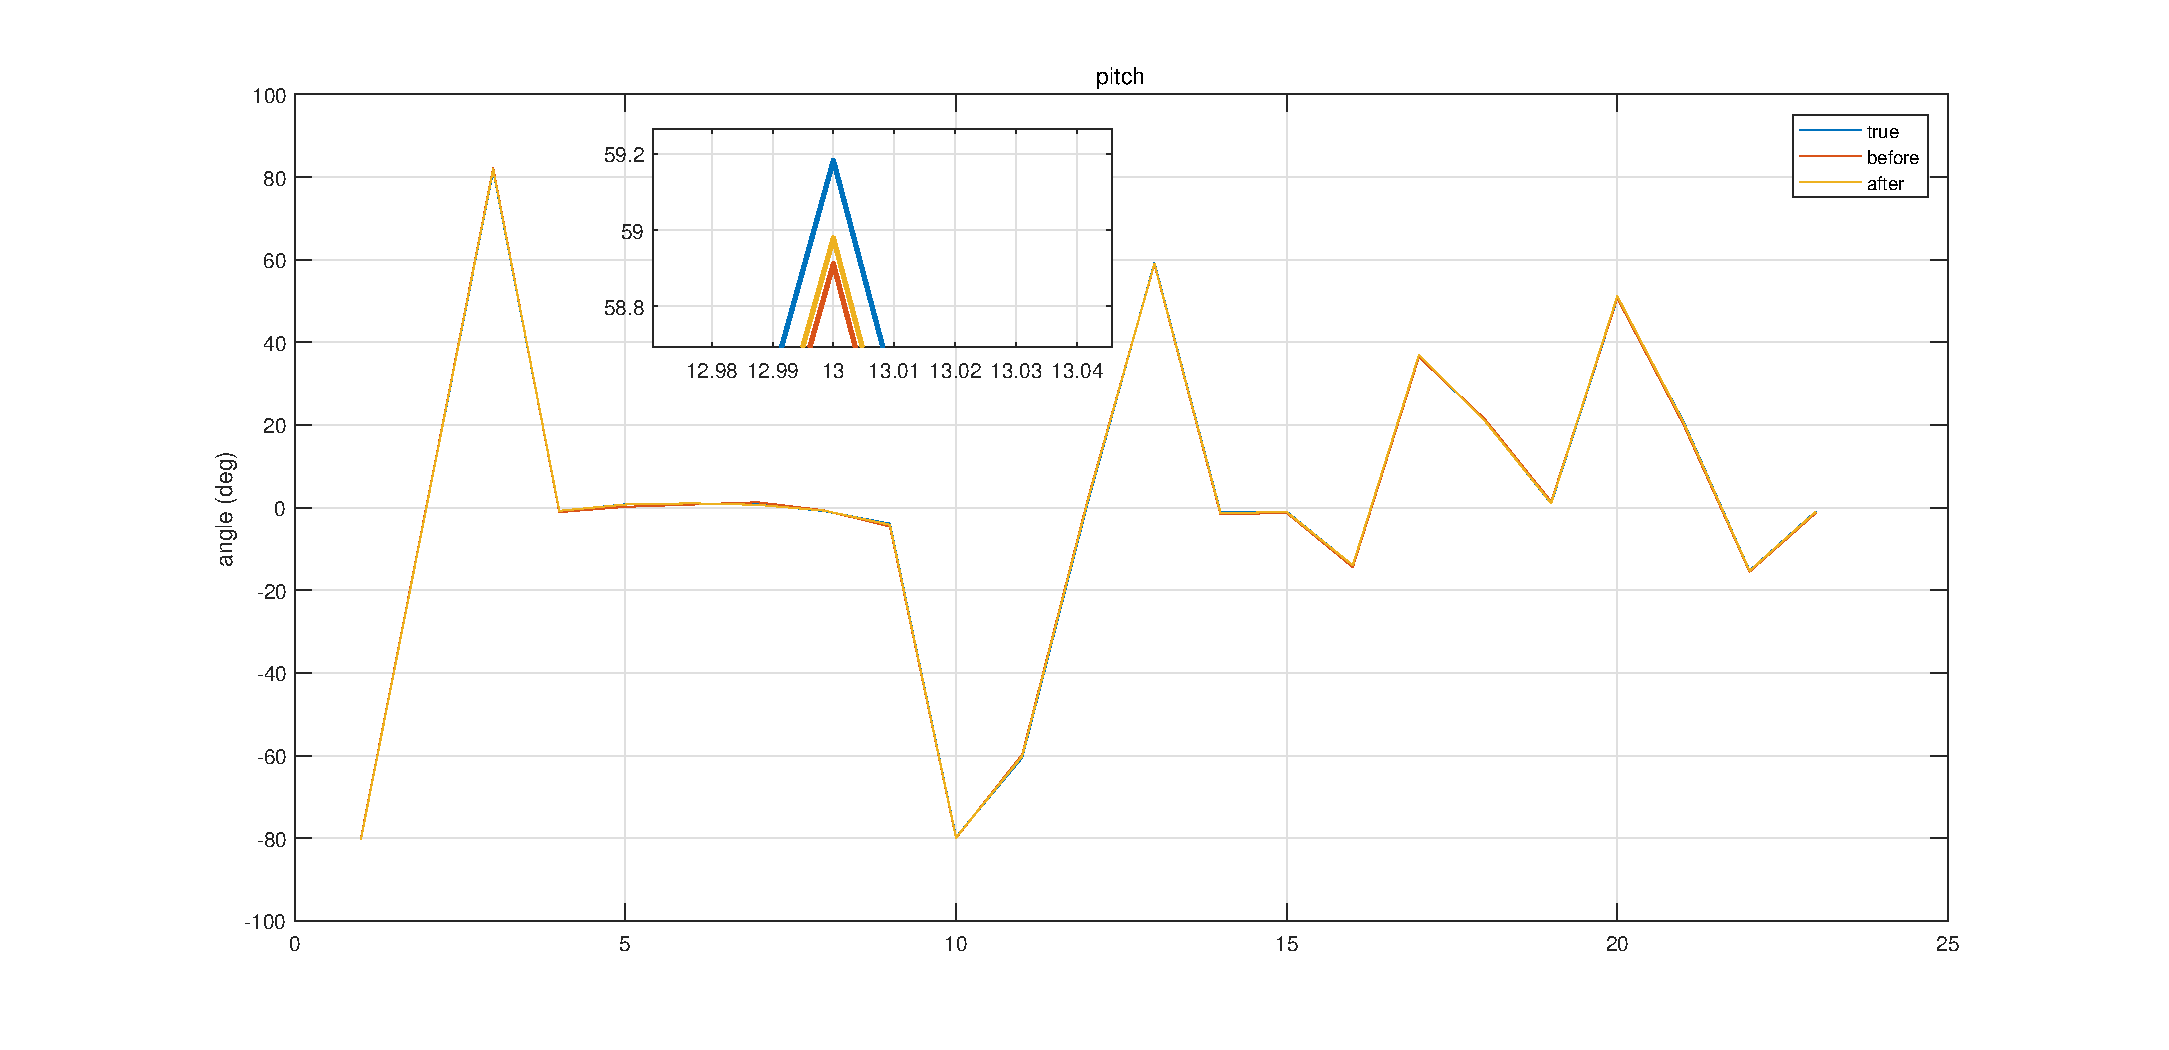
\includegraphics[width=1.0\textwidth]{piece.eps}
	\bicaption{分段姿态积分对比}{Piece attitude integral comparison}
	\label{fig:piece}
\end{figure}
第一个实验只对比每个区间终点姿态,真值由加速度计得到。
由\autoref{fig:piece}能看出,校准后的姿态更接近与真值。

第二个实验结果如\autoref{fig:full}
\begin{figure}[htbp]
	\centering
	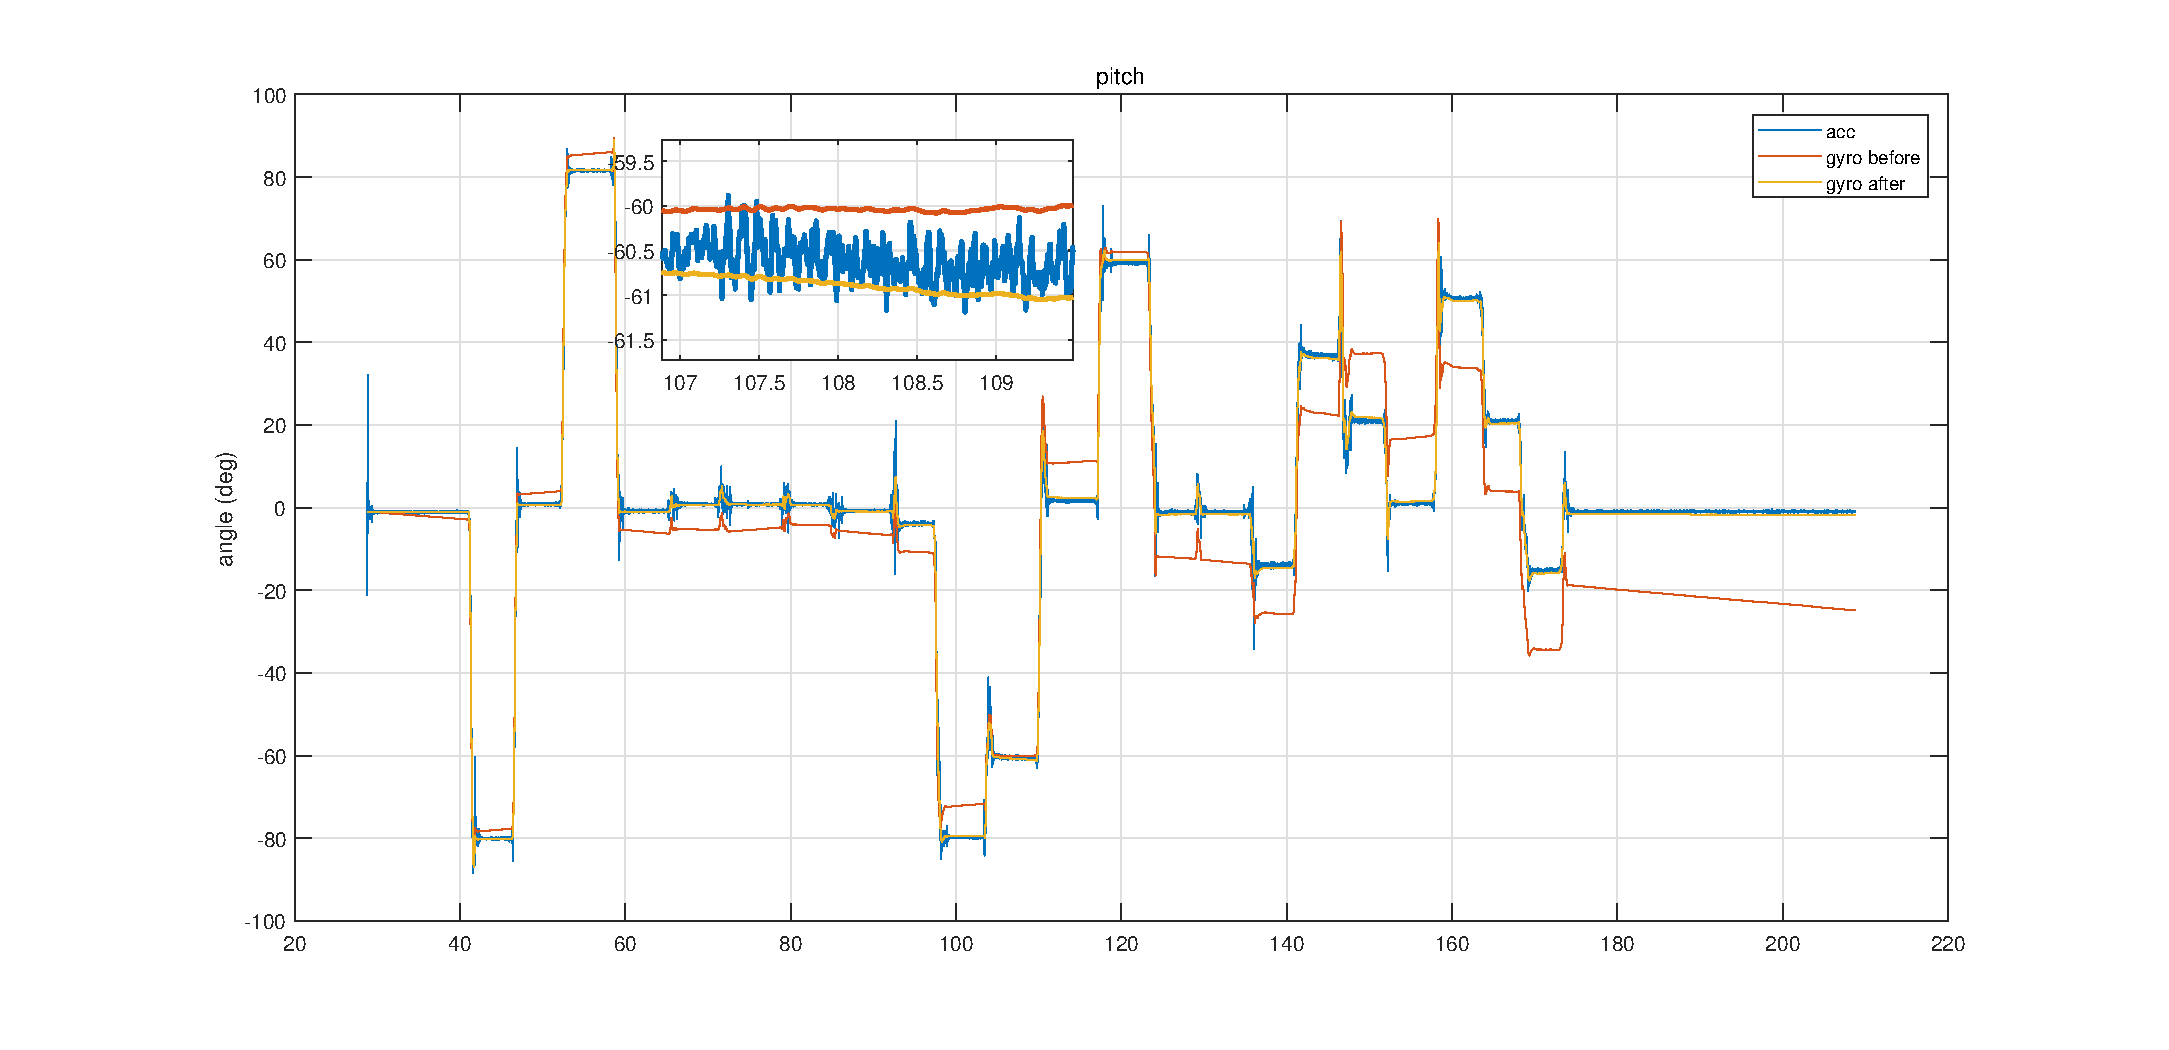
\includegraphics[width=1.0\textwidth]{full.eps}
	\bicaption{全程姿态积分对比}{Overall attitude integral comparison}
	\label{fig:full}
\end{figure}
第二个实验对比整个校准过程积分的姿态,真值由加速度计得到。
由\autoref{fig:full}能看出,校准后的姿态更接近与真值,并且无校准的姿态由于零偏误差较大。

我们给出陀螺仪校准的误差分析,如\autoref{gyrocaliberr}
\begin{table}[htbp]
	\bicaption{陀螺仪校准误差}{Gyroscope calibration error}
	\label{gyrocaliberr}
	\begin{tabular}{ccc}
		\toprule
		状态 & 平均误差$deg$ & 最大误差$deg$ \\
		\midrule
		校准前 & 1.4431 & 1.5965 \\
		校准后 & 0.1255 & 0.8970 \\
		\bottomrule
	\end{tabular}
\end{table}
其中,平均误差是陀螺仪短期积分的姿态与加速度计计算的姿态的差的平均值,最大误差是指所有陀螺仪短期积分的姿态与加速度计计算的姿态的差的最大值。
%\begin{table}[htbp]
%	\bicaption{IMU参数}{IMU parameters}
%	\label{IMUparameters}
%	\begin{tabular}{ccccccccccccc}
%		\toprule
%		传感器 & $\beta_{yz}$ & $\beta_{zy}$ & $\beta_{xz}$ & $\beta_{zx}$ & $\beta_{xy}$ & $\beta_{yx}$ & $s_x$ & $s_y$ & $s_z$ & $b_x$ & $b_y$ & $b_z$\\
%		\midrule
%		加速度计 & -0.0039 & 0.0081 & 0.0002 & -0.0037 & -0.0072 & 0.0047 & 0.9921 & 0.9963 & 0.9959 & 14.7897 & -7.4082 & 3.0406\\
%		陀螺仪 & 0.0081 & 0.0038\\
%		\bottomrule
%	\end{tabular}
%\end{table}

\gdutsubsection{算法对比}{Algorithm comparison}

\gdutsection{总结与讨论}{Summary and discussion}
在本章中,我们提出了一种IMU校准算法,该方法能够在无需外部设备的情况下进行校准。我们对校准评估标准方法的进行优化。我们的方法能够使精度提高到xxx。

\gdutchapter{多旋翼飞行器的控制算法设计}{Design of control algorithm for multi-rotor aircraft}
本章讨论如何设计控制算法,以配合飞行器稳定飞行的需要。
基于第二章的状态估计算法,控制器有800Hz的状态量作为反馈值。
通常这些测量值可以通过我们提出的状态估计算法得到。

\gdutsection{问题描述}{Problem formulation}
在对被控对象进行设计控制率之前,我们需要对被控对象进行建模。
对于我们的被控对象,需要对被控对象的动力学模型建立数学模型分析,以便我们综合设计系统。

\gdutsubsection{多旋翼飞行器动力学模型}{Dynamics model of multi-rotor aircraft}
考虑图\autoref{fig:modelaerialrobot}中所示的多旋翼飞行器模型。
这是一个由四个相同的电机和螺旋桨组成的系统。
通过螺旋桨产生的推力和扭矩垂直于飞行器所在平面。
我们选择了北东地(NED)坐标系作为世界坐标系,前右下坐标系作为机体坐标系。
机体坐标系的原点位于飞行器的质心。

基于这个模型,我们定义如下物理量

$m \in \mathbb{R}$,飞行器总质量;

$J \in \mathbb{R}^{3 \times 3}$,表示在机体坐标系下的转动惯量矩阵;

$R \in SO(3)$,从机体坐标系到世界坐标系的旋转矩阵;

$\omega^b \in \mathbb{R}^3$,表示在机体坐标系下的角速度;

$x \in \mathbb{R}^3$,表示在世界坐标系下的飞行器质心的位置;

$v \in \mathbb{R}^3$,表示在世界坐标系下的飞行器质心的速度;

$f \in \mathbb{R}$,螺旋桨沿电机轴产生的总推力;

$\tau \in \mathbb{R}^3$,表示在机体坐标系下的螺旋桨产生的总力矩;

基于以上定义,多旋翼飞行器的运动方程可以写成
%\begin{center}
\begin{gather}\label{eq:dynamics}
%\begin{equation}\label{eq:dynamics}
%	\begin{aligned}
		\dot{x} = v\\
		m\dot{v} = mge_3 - fRe_3\\
		\dot{R} = R\hat{\omega}^b\\
		J\dot{\omega}^b + \omega^b \times J \omega^b = \tau
%	\end{aligned}
%\end{equation}
\end{gather}
%\end{center}

\gdutsection{控制算法分析}{Control algorithm analysis}
在获得了飞行器的状态后,我们可以使用各种现有的控制策略使飞行器稳定飞行。
线性控制器,如PID控制器或LQR控制器,被广泛应用于多旋翼飞行器中\cite{hoffmann2007quadrotor,castillo2004stabilization,nice2004design}。
基于飞行器工作接近悬停状态的假设下,对于低速运行、加速度变化小的飞行器,可以使用线性控制器。
针对四旋翼无人机在饱和位置下的线性化动力学问题,Guenard等人设计了一种非线性控制器\cite{guenard2005dynamic}。
文献\cite{bouabdallah2005backstepping}中应用了反步和滑模技术。
因为这些控制器是基于欧拉角设计的,它们在表示多旋翼飞行器复杂的旋转运动时表现出奇点,从而从根本上限制了它们跟踪轨迹的能力。
基于李群上的刚体动力学描述,Lee等人设计了一种应用在四旋翼飞行器的几何控制器,并证明了几乎全局稳定性\cite{lee2010geometric}。
对于包含大姿态变化的运动,文献\cite{lee2010geometric}的控制器是更合适的选择。
我们基于\cite{lee2010geometric}的设计控制系统。

\gdutsection{控制算法设计}{Control algorithm design}
我们设计了一个控制器跟踪轨迹。
我们直接针对非线性耦合系统设计控制器。

\gdutsubsection{控制框架设计}{Control scheme design}
控制器总体框架如\autoref{fig:controllerstructure}所示。
\begin{figure}[htbp]
	\centering
	\includegraphics[width=1.0\textwidth]{屏幕截图 2022-04-04 222027.png}
	\bicaption{控制框架图}{Controller structure}
	\label{fig:controllerstructure}
\end{figure}
运动方程\autoref{eq:dynamics}具有级联结构。
姿态的转动运动与平动运动解耦。
平动只依赖于公式(4.3)中的$fRe_3$项。
总推力$f$的大小是直接控制的,而总推力$Re_3$的方向是由机体轴$\vec{b}_3$决定的。
因此,为了改变总推力的方向,应相应地改变姿态。
这里,我们选择所需的总推力$f$以及目标姿态$R_d e_3$作为输入跟踪位置$x_d$。
控制力矩$\tau$作为输入跟踪目标姿态$R_d$。

\gdutsubsection{控制率设计}{Control law design}
根据\autoref{fig:controllerstructure}展示的控制框架,控制器可以分为位置控制器和姿态控制器两部分。

对于位置控制器,我们直接针对非线性耦合系统设计控制器。
这种类型的位置控制器最终产生的目标值为旋转矩阵$R_d$和拉力$f$。
我们将位置控制器解耦成水平控制器和高度控制器。水平控制器输出目标姿态$R_d$,高度控制器输出推力$f$。

对于目标姿态的生成,根据文献\cite{lee2010geometric}给出的控制律为
\begin{gather}\label{eq:Horizontalcontrol}
	\vec{b}_{3d} = -\frac{-k_x e_x - k_v e_v - mge_3 + m\ddot{x}_d}{\left\|-k_x e_x - k_v e_v - mge_3 + m\ddot{x}_d\right\|}
\end{gather}
其中,$\vec{b}_{3d}$是期望机体系z轴在世界坐标系的表示,由z轴的坐标我们能根据几何关系算出目标横滚角$\phi_d$和目标俯仰角$\theta_d$,加上直接给定的目标偏航角$\psi_d$可以得到$R_d$。

对于推力的生成,根据多旋翼飞行器的结构,控制率为
\begin{gather}\label{eq:AltitudeControl}
	f = -\frac{ma_d + f_0 cos\theta_0 cos\phi_0}{cos\theta cos\phi}
\end{gather}
其中,$f_0 cos\theta_0 cos\phi_0$表示了悬停油门。

对于姿态控制器,根据文献\cite{yu2015high}给出的稳定控制律为
\begin{equation}\label{eq:attitudecontrol}
	\tau = \omega^b \times J \omega^b + K_p log(R_e)^{\vee} - K_d \omega^b_e
\end{equation}
注意到$log(R_e)$可以看作是目标角速度$\omega^b_d$。
\autoref{eq:attitudecontrol}中的第二项和第三项可以分开控制。

角速度控制
\begin{gather}\label{eq:angularacontrol}
	\omega^b_e = log(R_e)^{\vee} - \omega^b\\
	\dot{\omega}^b_d = K_p \omega^b_e
\end{gather}

角加速度控制
\begin{gather}\label{eq:angularaccelerationcontrol}
		\dot{\omega}^b_e = \dot{\omega}^b_d - \dot{\omega}^b\\
		\tau = K_p \dot{\omega}^b_e + K_i \int_{0}^{t}\dot{\omega}^b_e + \omega^b \times J \omega^b
\end{gather}

\gdutsection{实验结果}{Experimental results}
我们有一个基于多传感器融合的状态估计器来产生800Hz的位置、速度、姿态估计,足以稳定飞行器。

实验中,我们随意遥控飞行器前后左右飞行,记录机体姿态的实际响应情况。
以下是测试结果。

\begin{figure}[htbp]
	\centering
	\includegraphics[width=0.7\textwidth]{屏幕截图 2022-04-06 150427.png}
	\bicaption{横滚与俯仰跟踪结果}{Roll and pitch tracking results}
	\label{fig:Rptrackingresults}
\end{figure}

\begin{figure}[htbp]
	\centering
	\includegraphics[width=0.7\textwidth]{屏幕截图 2022-04-06 151409.png}
	\bicaption{横滚与俯仰控制输出}{Roll and pitch control output}
	\label{fig:Rpcontroloutput}
\end{figure}

从\autoref{fig:Rptrackingresults}中可看到:
(1)姿态有一定的超调,但是超调后的回复过程是平稳的。
(2)观察控制俯仰角跟踪-30°期望角度时的结果可以看出,我们的算法存在一些稳态误差,后续可通过积分设计改善;
(3)整体控制输出较为平滑,可以满足实际飞行需求。

\gdutsection{总结与讨论}{Summary and discussion}
在本章中,我们整合了现有的控制算法,完成了整个飞行控制系统的闭环,实现飞行器的稳定飞行。

\gdutbackmatter
\gdutchapter{结论与展望}{Conclusion and prospect}
在这篇论文中,我们展示了对飞行器自主飞行的最新技术的贡献,大部分贡献是状态估计算法。在第三章中,我们开发了状态估计系统,提出了一种模块化和可扩展的方法,该方法能够以一致的方式组合来自多个传感器的信息。在第四章中,我们开发了传感器校准算法,能够在没有外部设备的情况下对传感器进行高精度的校准。在第五章中,我们提出的控制方法结合前两章的算法形成一个集成的飞行器系统。

我们注意到,虽然主要的实验平台使用的是四旋翼,但我们的方法不限于这一特定类型的平台。实际上,我们的方法是基于传感器的,同样适用于其他机器人,如固定翼、地面机器人等。
\gdutbacksection{成果总结}
综上所述,本文的主要贡献如下:
\begin{itemize}
	\item 我们开发了算法和系统,使计算资源受限的飞行器能够自主飞行,只使用低成本的传感器。
	\item 我们提出了一种算法,通过互补融合来自多传感器的信息来提高系统的可靠性。
	\item 我们提出了一种算法,无需外部设备就能够进行传感器校准。
	\item 我们开发集成了控制算法,并通过大量的实验表明,飞行控制系统是稳定可靠的。
\end{itemize}

\gdutbacksection{未来研究展望}
本文涉及到了几个有趣的研究领域,其中一些是随着飞行器技术的发展而不断发展成大型系统的,而另一些则是我们在评估最新方法的性能时值得追求的新方向。
\paragraph{自主飞行中估计与控制的耦合设计。}
在我们目前的工作中,控制器与估计器是分开设计的。然而,随着我们朝着高速自主飞行的方向发展,我们可能会要求估计器和控制器耦合设计,以生成和执行高效、无碰撞和安全的飞行轨迹。
\paragraph{用于飞行器的新的传感器技术。}
虽然传统的传感器如IMU、GPS、相机已被证明可用于飞行器导航,但最近传感技术的发展可能创造新的机会。例如,光场可以作为深度感知的传感器。这些新型传感技术在飞行器上的应用具有很大的潜力。
\paragraph{传感器和能观性研究。}
众所周知,传感器数量越多,系统的能观性越好,但单个传感器对系统能观性的影响尚不清楚。增加更多的传感器会带来出更多的能观性,但是传感器提供的信息以及信息的质量会导致能观性的复杂判断条件。因此,一个能够以在线方式识别能观性的通用框架将有利于更高层次的任务,如运动规划和风险评估。

\nocite{*}% 列出全部参考文献
\printbibliography

\gdutchapter{攻读学位期间取得与学位论文相关的成果}{Publication and patents during study}

\gdutbacksection{发表和投稿与学位论文相关学术论文}

\begin{results}
  \item \textbf{张三}, 李四, 等. Jet electrochemical machining of micro dimples with conductive mask.
  Journal of Materials Processing Technology. 2018, 257:101-111. (SCI Impact Factor 3.647,
  WOS:000431161400010)
  \item 李四, \textbf{张三}, 王五, 等. Electrochemical direct-writing machining of micro- channel array.
  Journal of Materials Processing Technology. 2019, 265:138-149. (SCI Impact Factor 3.647,
  WOS:000451935100014)
\end{results}

\gdutbacksection{申请发明专利}

\begin{results}
  \item 李四, \textbf{张三}, 王五. 一种微流道电解加工装置. 发明专利申请号: 201810467763.5.
\end{results}

\gdutstatement

\gdutchapter{致谢}{Acknowlegements}
\zhlipsum[1]

\gdutappendix

\gdutchapter{附录标题}{The appendix title}
对需要收录于学位论文中且又不适合书写于正文中的附加数据、资料、详细
公式推导、计算机程序等有特色的内容,可做为附录排写。
\end{document}